\documentclass[11pt]{article}

\usepackage{latexsym}
\usepackage{amsmath}
\usepackage{amssymb}
\usepackage{amsthm}
\usepackage{graphicx}
\usepackage{wrapfig}
%\usepackage{pseudocode}
\usepackage{url}
\usepackage{subfig}
\usepackage[backref, colorlinks=true, citecolor=red, urlcolor=blue, pdfauthor={Jyh-Ming Lien}]{hyperref}


\newcommand{\handout}[5]{
  \noindent
  \begin{center}
  \framebox{
    \vbox{
      \hbox to 5.78in { {\bf } \hfill #2 }
      \vspace{4mm}
      \hbox to 5.78in { {\Large \hfill #5  \hfill} }
      \vspace{2mm}
      \hbox to 5.78in { {\em #3 \hfill #4} }
    }
  }
  \end{center}
  \vspace*{4mm}
}

\newcommand{\lecture}[4]{\handout{#1}{#2}{#3}{#4}{#1}}

\newtheorem{theorem}{Theorem}
\newtheorem{corollary}[theorem]{Corollary}
\newtheorem{lemma}[theorem]{Lemma}
\newtheorem{observation}[theorem]{Observation}
\newtheorem{proposition}[theorem]{Proposition}
\newtheorem{definition}[theorem]{Definition}
\newtheorem{claim}[theorem]{Claim}
\newtheorem{fact}[theorem]{Fact}
\newtheorem{assumption}[theorem]{Assumption}

% 1-inch margins, from fullpage.sty by H.Partl, Version 2, Dec. 15, 1988.
\topmargin 0pt
\advance \topmargin by -\headheight
\advance \topmargin by -\headsep
\textheight 8.9in
\oddsidemargin 0pt
\evensidemargin \oddsidemargin
\marginparwidth 0.5in
\textwidth 6.5in

\parindent 0in
\parskip 1.5ex
%\renewcommand{\baselinestretch}{1.25}

\begin{document}

\lecture{Final Project Report: Hubness and Some Questions}{Fall 2017}{Yimeng Li and Vega Bharadwaj}{CS 584 Data Mining}

\section{Introduction}
The number of k-occurences of point $x$ from dataset $D$ is called its hubness score. High hubness score indicates that this point is close to plenty of other points in the dataset. In a regular clustering algorithm, e.g. K-Means, a cluster medoid is also the point closest to all the points in the cluster. Since both of them, a cluster medoid and a high hubness point, share the same attribute, we believe it's highly possible that high hubness points are more likely to become cluster medoids comparing to points with a lower hubness score. In this project, we unveil the relationship between high hubness points and cluster medoids on both synthetic and real-world datasets.\\
Besides, low hubness scores also indicates that a point is far away from the majority of its peers, which is big sign of being an outlier or a noise. We happened to learn an algorithm called DBSCAN during the semester, which is quite effective in finding data outliers using density information. The second problem we are trying to solve is to explore the relation between low hubness points and DBSCAN-detected noise points on both synthetic and real-world datasets.

\section{Related Work}
Hubness has been observed in several fields of applications involving sound and image data during recent years (Aucouturie and Pachet, 2007; Doddington et al., 1998; Hicklin et al., 2005) and, in addition, Jebara et al. Hubness phenomenon in the construction of the neighborhood graph of learning (Tony Jebara et al 2009) [2]. Amina M et al. designed a hubness-based algorithm by introducing hubs into the k-means algorithm (Amina M et al 2015) [3]. Although people does not give much attention to the phenomenon of hubness in data clustering, the k-nearest-neighbor list is widely used in many clusters. The k-nearest-neighbor list computes the density estimate by the volume used to observe the space determined by the k nearest neighbors. Density-based clustering methods generally rely on this density estimation. The main goal of density-based clustering algorithms is to find high-density areas separated by low-density areas [4]. In high-dimensional space, this is often difficult to estimate because data is usually sparse. It is also important to choose the appropriate neighborhood size, because too small or too large k values ​​may cause the density-based approach to fail. The k-nearest-neighbor list is often used to construct k-NN graphs and so it's used in graph clustering. 

\section{Solutions}
To explore the relation between hubs and clusters, we did experiments on both synthetic datasets and real-world datasets. All the experiments are finished using MATLAB.\\
First part of the experiment is performed on the synthetic datasets. We run K-Means on each gaussian mixture. The K-Means algorithm is initialized by using K-Means++. In each iteration, we measure the distance from each cluster centroid to its closest neighbor and to the strongest hub inside the cluster, and scaled by the average intracluster distance. Both minimal and maximal distance among all the clusters are computed. We run the whole process several times and compute the average minimal and maximal distances to eliminate the noise brought in by K-Means random initialzation. In the end we compare the average minimal distance to a medoid and to a strong hubness point to see if they are the same point. And of course we also compare the maximal distances between them. Second part of the experiment is done on the real-world datasets. Before we running the real algorithms on these datasets, we first do some data preprocessing. For each point in a dataset, we normalize its attributes values across the whole dataset using minmax normalization. Then we go through the same computing process on each real dataset as we do on the gaussian mixtures. \\Even though we implement all the experiments by ourselves, it's worth mentioning how we find the strongest hubness point in each cluster. We first call $knnsearch()$ function to find the nearest neighbors of each point in the cluster. Then we call $unique()$ function to pick out points that are the neighbors of other points. $histc()$ function is called to figure out the number of times each point being the nearest neighbor of other points. The point with the largest number is the strongest hubness point in the dataset. To compute the intraclass distance, we call $pdist2()$ function to compute the euclidean distance from each point in the cluster to the centroid. We sum up these distances and divide it by the number points in the cluster to get the intraclass distance. The cluster medoid is found by seeing the point which has the smallest distance to the cluster centroid.\\
To explore the relation between hubs and DBSCAN outliers, experiments are also finished using both synthetic datasets and real-world datasets.First part of the experiment is done on the synthetic datasets. We run DBSCAN on each gaussian mixture to find the outliers. The $eps$ value, the radius of each core circle, is set up manually by reading the kdist graph of the whole dataset. Then we compute the hubness score of all the points in the dataset. For the DBSCAN detected noise points, we check if their hubness scores are two standard deviations lower than the average hubness value of all the points. Second part of the experiment is done on the real-world datasets. We still need to manually set up the eps value. Then we do the same comparison between the outliers’ hubness scores and the average hubness value.\\
How we find the strongest hubness point in the dataset is the same as what we do when we find the relationship between hubs and cluster medoids. The difference is that in the hubs and medoids experiment, we find the strongest hubness point of each cluster. The hubness point is computed by finding each point's nearest neighbors inside the cluster. But in the hubs and DBSCAN noise points experiment, each point's hubness score is decided by each point's nearest neighbors over the whole dataset, rather than just points in the same cluster. To compute the average and standard deviation of the hubness scores, we call MATLAB functions $mean()$ and $std()$ respectively.

\section{Experiments}
\subsection{Data}
Two types of data are including synthetic and real-world data sets.\\
For synthetic datasets, we create 7 random generated gaussian mixtures by using $gmdistribution()$ from MATLAB. All the gaussian mixtures are generated from a given list of dimensions: 2, 5, 10, 20, 30, 50, 100 and are created from 10 Gaussian generators. So each mixture has 10 clusters. When we create the mixtures, the gaussian distribution mean is uniformly chosen from $[lower\_bound^{\mu}, upper\_bound^{\mu}]^{dimension}$, $lower\_bound^{\mu}=-20$, $upper\_bound^{\mu}=20$ and the standard deviations is also randomly chosen from $[lower\_bound^{\sigma}, upper\_bound^{\sigma}]^{dimension}$, $lower\_bound^{\sigma}=2$, $upper\_bound^{\sigma}=5$. And we randomly generate 10000 points for each mixture.\\
For the real world datasets, we take several datasets from UCI dataset repository. And they are described in an ascending order of their dimension.
\begin{itemize}
\item Iris Dataset. It is perhaps the best known database to be found in the pattern recognition literature. It has 150 instances and the data dimension is 4 and it has 3 classes. It can be downloaded from \url{https://archive.ics.uci.edu/ml/datasets/iris}.
\item Abalone Dataset. The data comes from predicting the age of abalone from physical measurements. It has 4177 instances and the data dimension is 8 and it also has 8 classes. It can be downloaded from \url{https://archive.ics.uci.edu/ml/datasets/abalone}.
\item Breast Cancer Wisconsin (Prognostic) Dataset. Each record represents follow-up data for one breast cancer case. It has 198 instances and the data dimension is 32 and it has 2 classes. It can be downloaded from \url{https://archive.ics.uci.edu/ml/datasets/Breast+Cancer+Wisconsin+(Prognostic)}.
\item Sonar Dataset. The data is obtained by bouncing sonar signals off a metal cylinder at various angles and under various conditions. It has 208 instances and the data dimension is 60 and it has 2 classes. It can be downloaded from \url{http://archive.ics.uci.edu/ml/datasets/connectionist+bench+(sonar,+mines+vs.+rocks)}.
\item Hill-Valley Data Set. Each record represents 100 points on a two-dimensional graph. When plotted in order as the Y co-ordinate, the points will create either a Hill or a Valley. It has 606 instances and the data dimension is 100 and it has 2 classes. It can be downloaded from \url{http://archive.ics.uci.edu/ml/datasets/hill-valley}.
\end{itemize}

\subsection{Experiment Setup}
To make sure that the implementation computing hubness scores is correct, we replicate the experiment settings mentioned in [1] to see if I get similar results.\\
To evaluate our experiments on hubs distribution across clusters, we will draw some plots to show how the maximal distance and minimal distance evolve through iterations. Data dimensions below 10 are used to illustrate low-dimensional behavior while dimensions above 10 are used to illustrate high-dimensional behavior. The neighborhood size is set to 10 across all the datasets.\\
To set up the DBSCAN $eps$ parameter, we read the kdist graph, a graph recording the distance of each point to its 10th nearest neighbor. Table \ref{tab:exp-setup} shows the $eps$ value of each dataset.
\begin{table}
\begin{center}
	\begin{tabular}{||c c c c||}
	\hline
	Synthetic Datasets & Eps Value & Real Datasets & Eps Value\\[0.5ex]
	\hline
	2-dim gm & 1.0 & Iris & 0.28\\
	\hline
	5-dim gm & 3.2 & Abalone & 0.17\\
	\hline
	10-dim gm & 5.8 & WPBG & 1.2\\
	\hline
	20-dim gm & 9.3 & Sonar & 2.2\\
	\hline
	30-dim gm & 12.0 & Hill and Valley & 0.8\\
	\hline
	50-dim gm & 16.5 &  & \\
	\hline
	100-dim gm & 24.6 &  & \\
	\hline
\end{tabular}
\caption{Datasets and DBSCAN $eps$ Parameter}
\end{center}
\label{tab:exp-setup}
\end{table} 

\subsection{Experimental Results}
\begin{figure}[ht]
	\begin{center}
		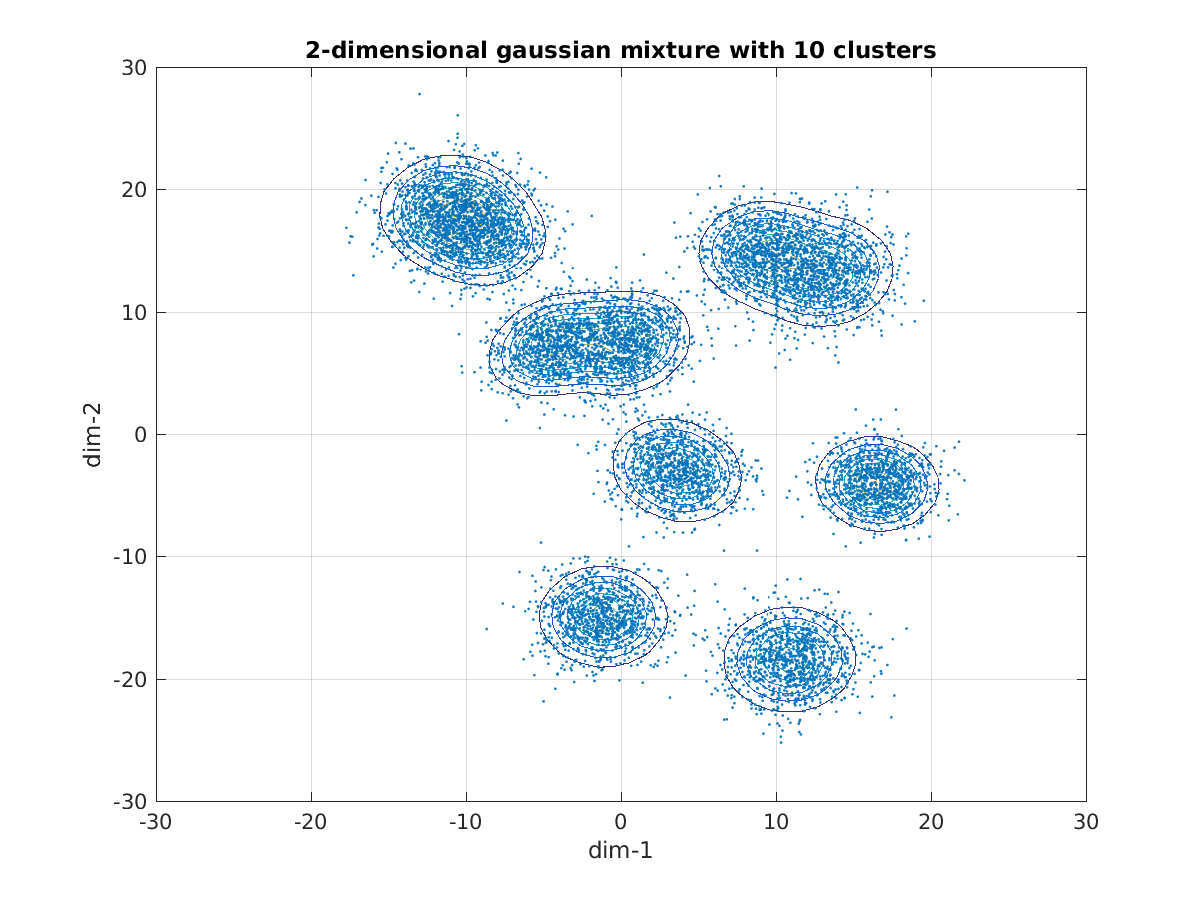
\includegraphics[width=0.8\textwidth]{FIGS/example_gaussian_mixture.png}
		\caption{Example Gaussian Mixture}
		\label{fig:example_gm}
	\end{center}
\end{figure}

% synthetic dataset min and max distances of lower dimension
\begin{figure}[ht]
	\begin{center}
		\subfloat[Minimal dis, d = 2]{
			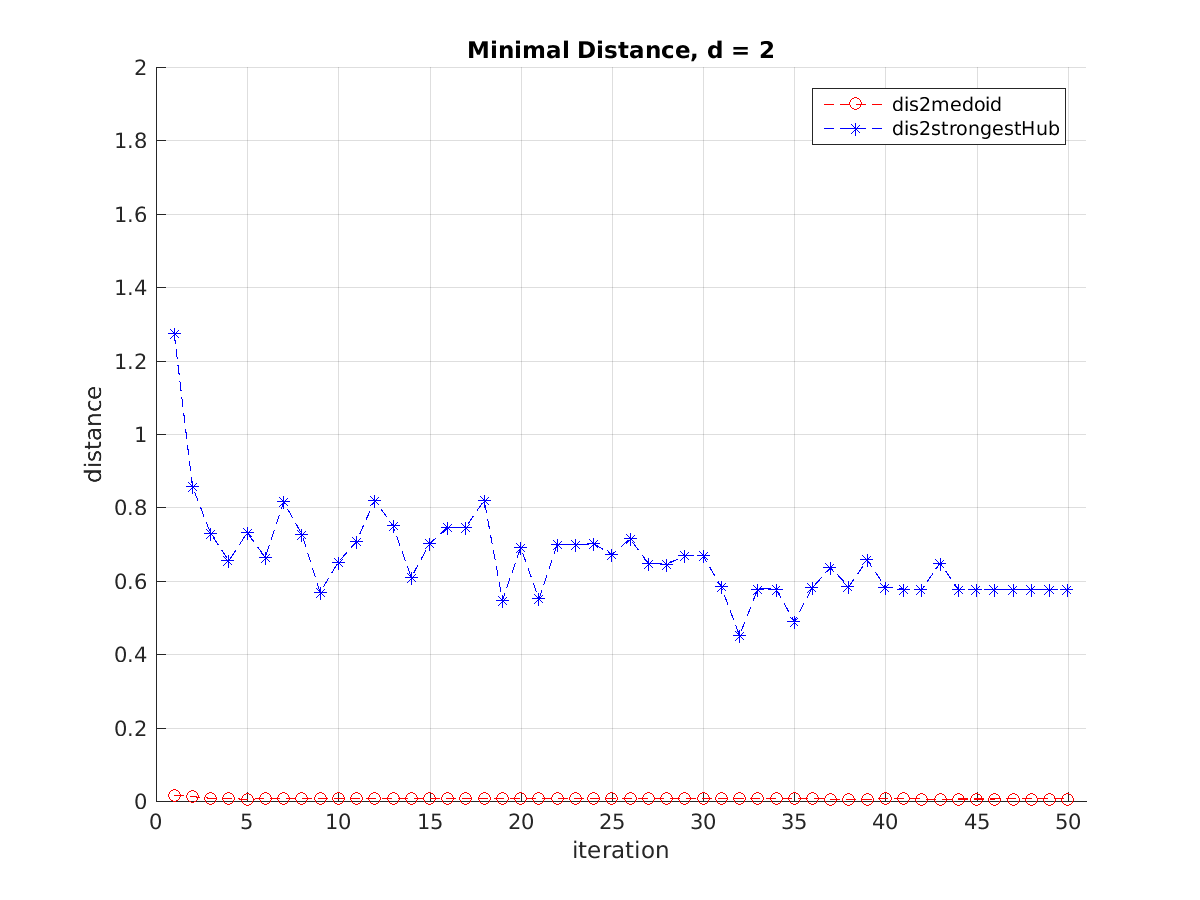
\includegraphics[width=0.4\textwidth]{FIGS/part1-synData/dim2_avg_min.png}
		}
		\hspace{5mm}
		\subfloat[Maximal dis, d = 2]{
			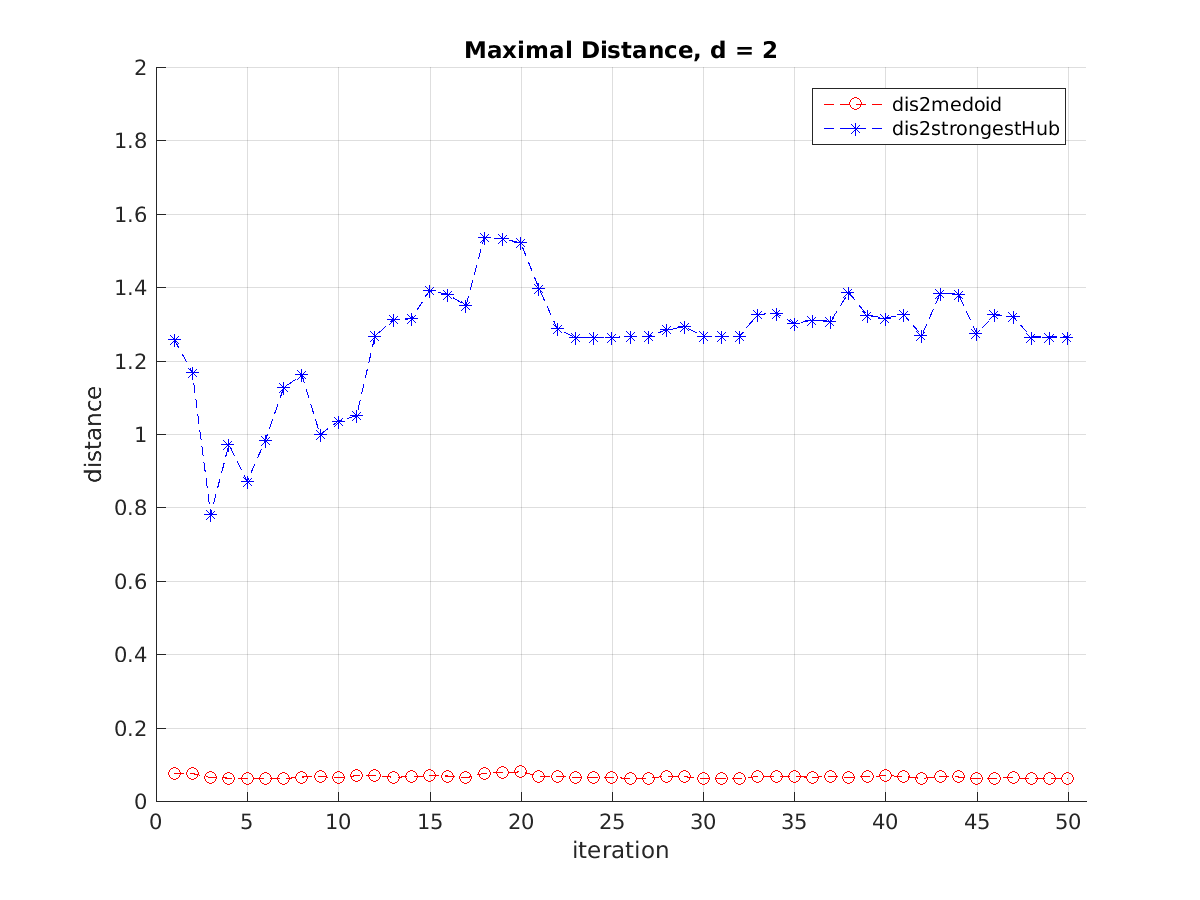
\includegraphics[width=0.4\textwidth]{FIGS/part1-synData/dim2_avg_max.png}
		}
		\hspace{5mm}
		\subfloat[Minimal dis, d = 5]{
			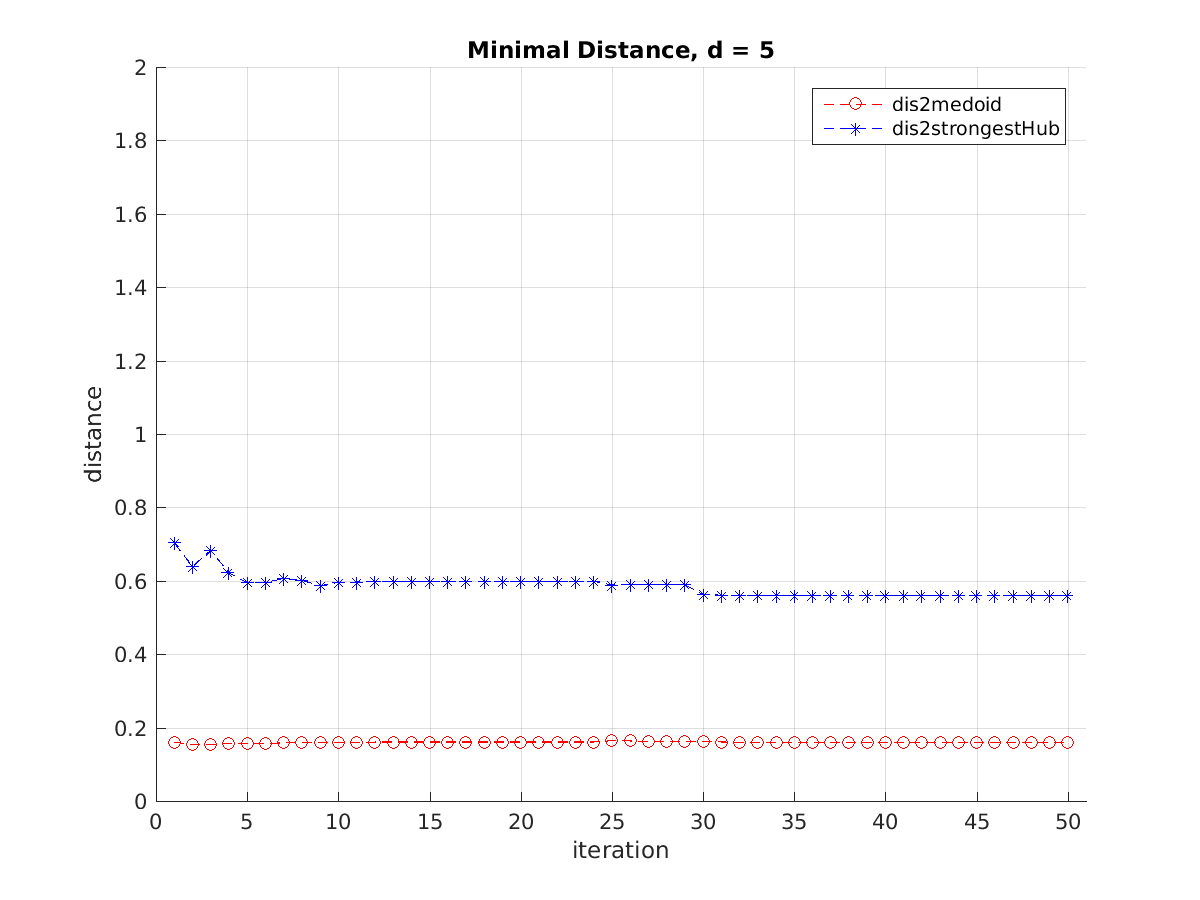
\includegraphics[width=0.4\textwidth]{FIGS/part1-synData/dim5_avg_min.png}
		}
		\hspace{5mm}
		\subfloat[Maximal dis, d = 5]{
			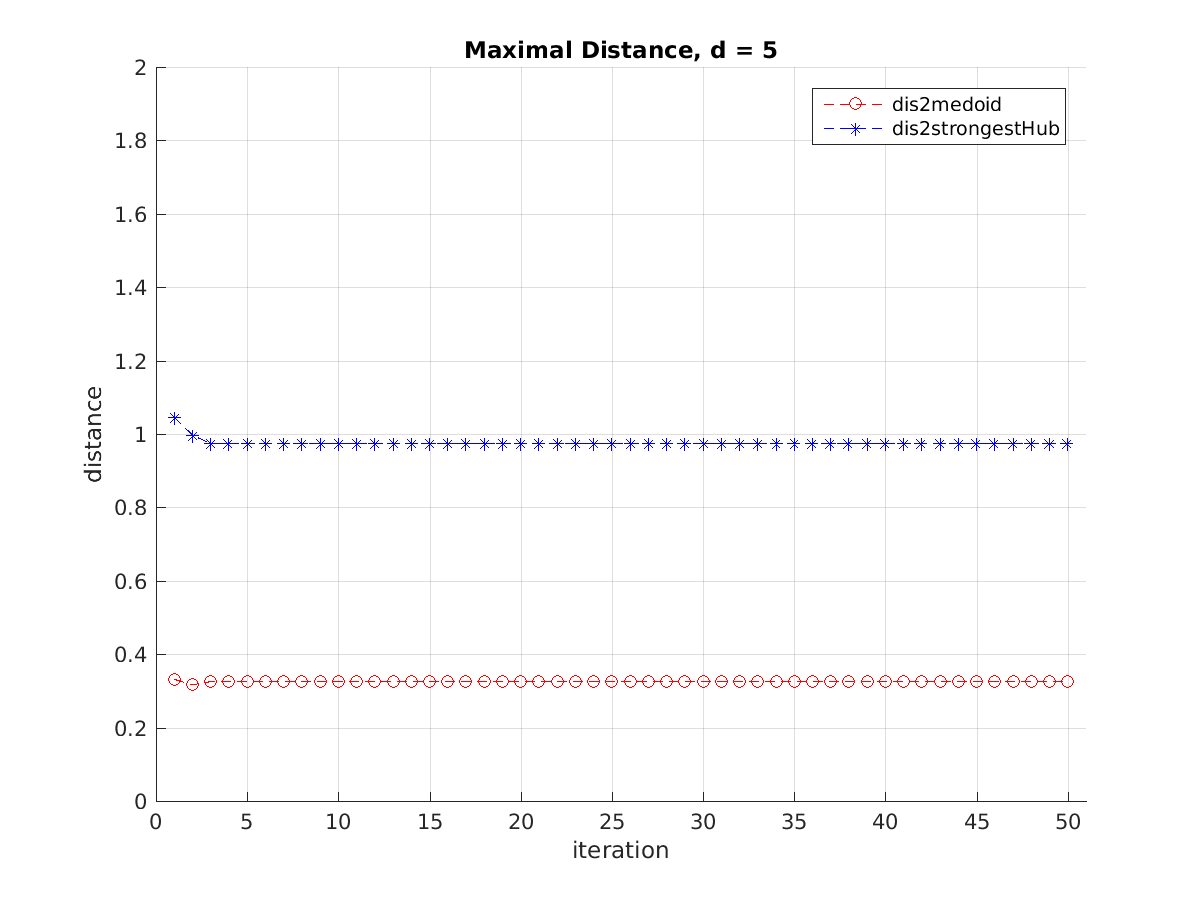
\includegraphics[width=0.4\textwidth]{FIGS/part1-synData/dim5_avg_max.png}
		}
		\hspace{5mm}
		\subfloat[Minimal dis, d = 10]{
			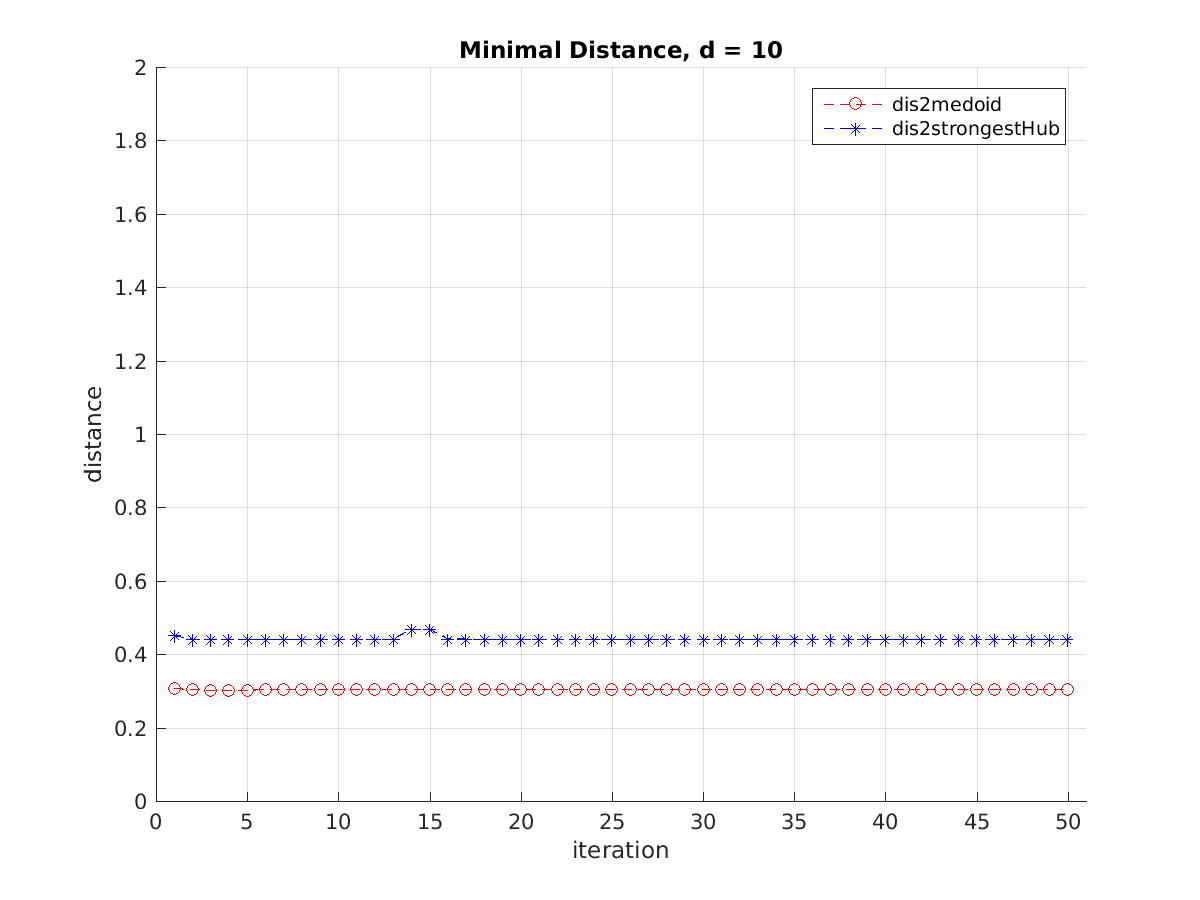
\includegraphics[width=0.4\textwidth]{FIGS/part1-synData/dim10_avg_min.png}
		}
		\hspace{5mm}
		\subfloat[Maximal dis, d = 10]{
			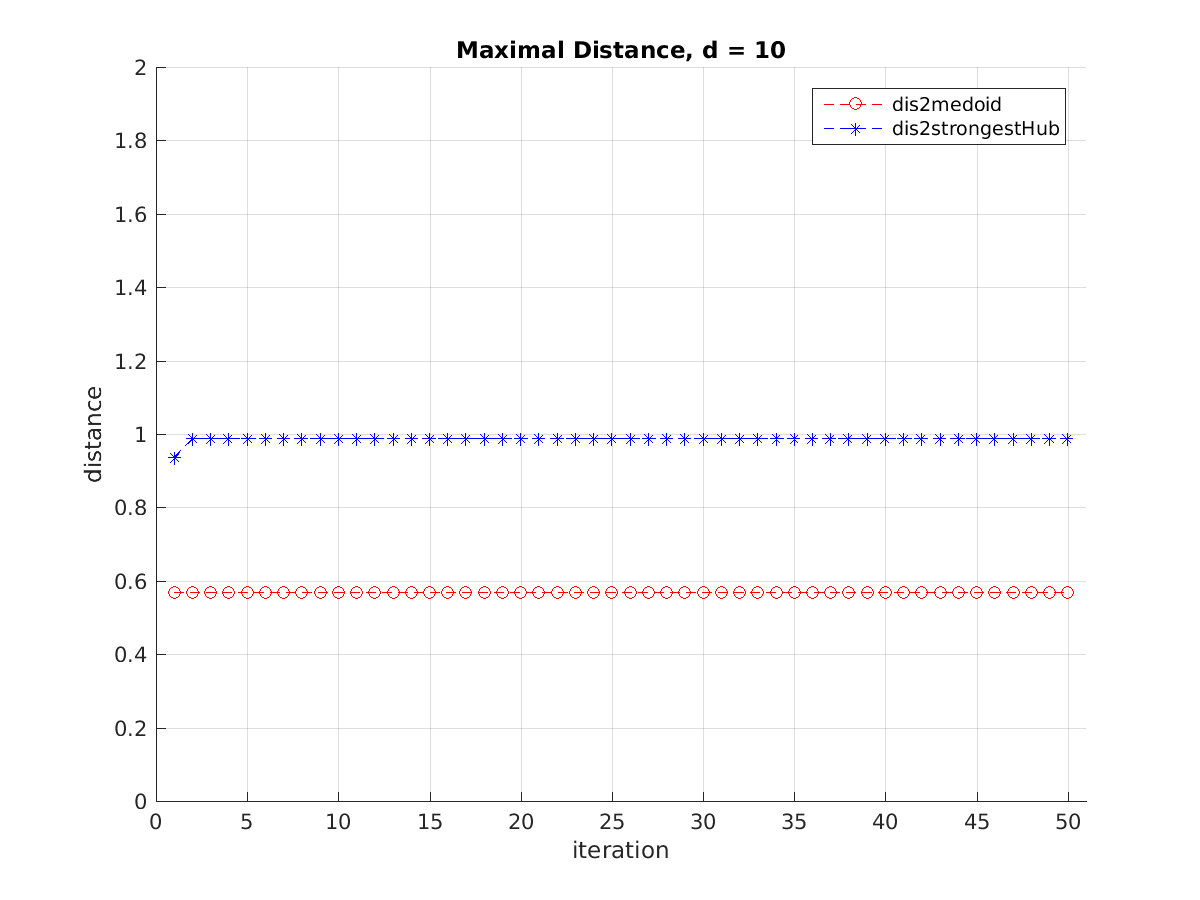
\includegraphics[width=0.4\textwidth]{FIGS/part1-synData/dim10_avg_max.png}
		}
		\caption{low-dim synthetic data results}
	\label{fig:syn1}
	\end{center}
\end{figure}
% synthetic dataset min and max distances of higher dimension
\begin{figure}[ht]
	\begin{center}
		\subfloat[Minimal dis, d = 20]{
			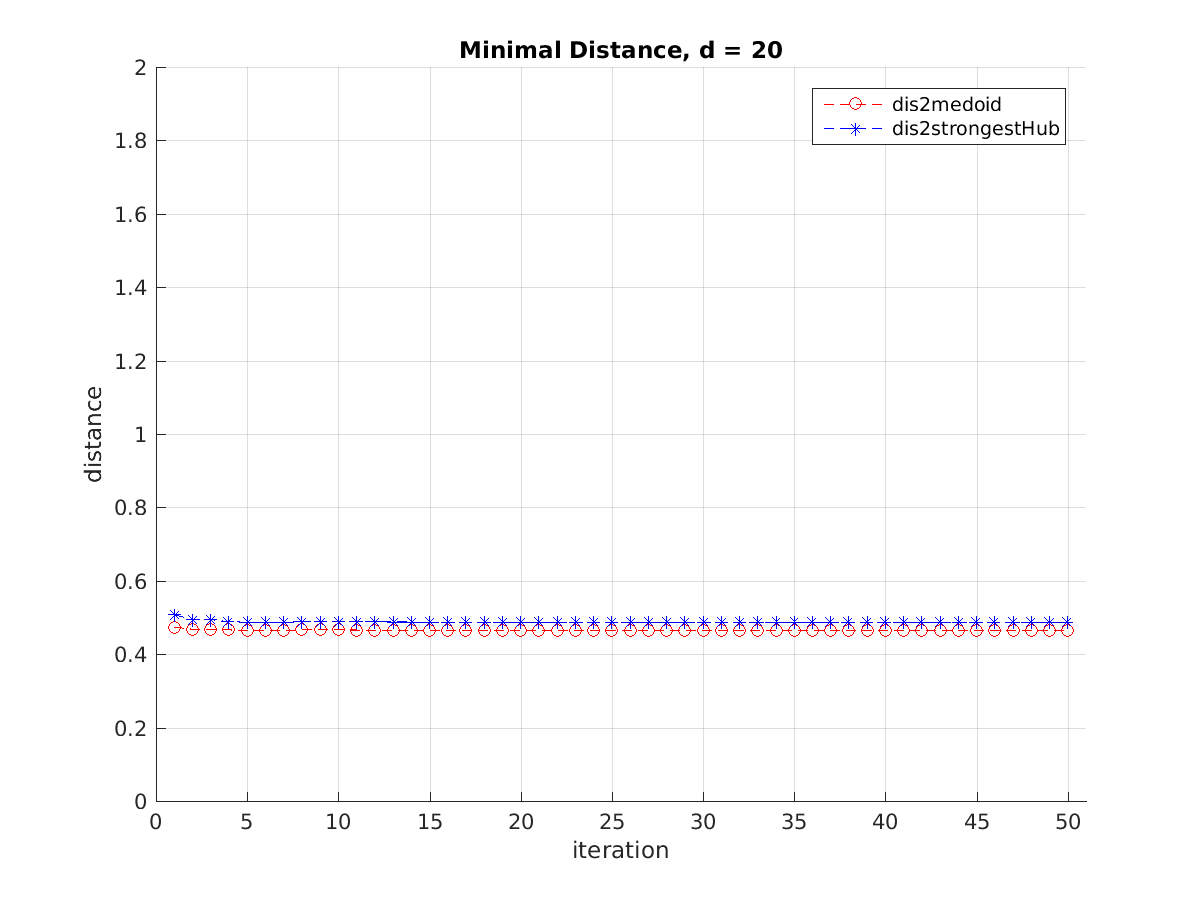
\includegraphics[width=0.4\textwidth]{FIGS/part1-synData/dim20_avg_min.png}
		}
		\hspace{5mm}
		\subfloat[Maximal dis, d = 20]{
			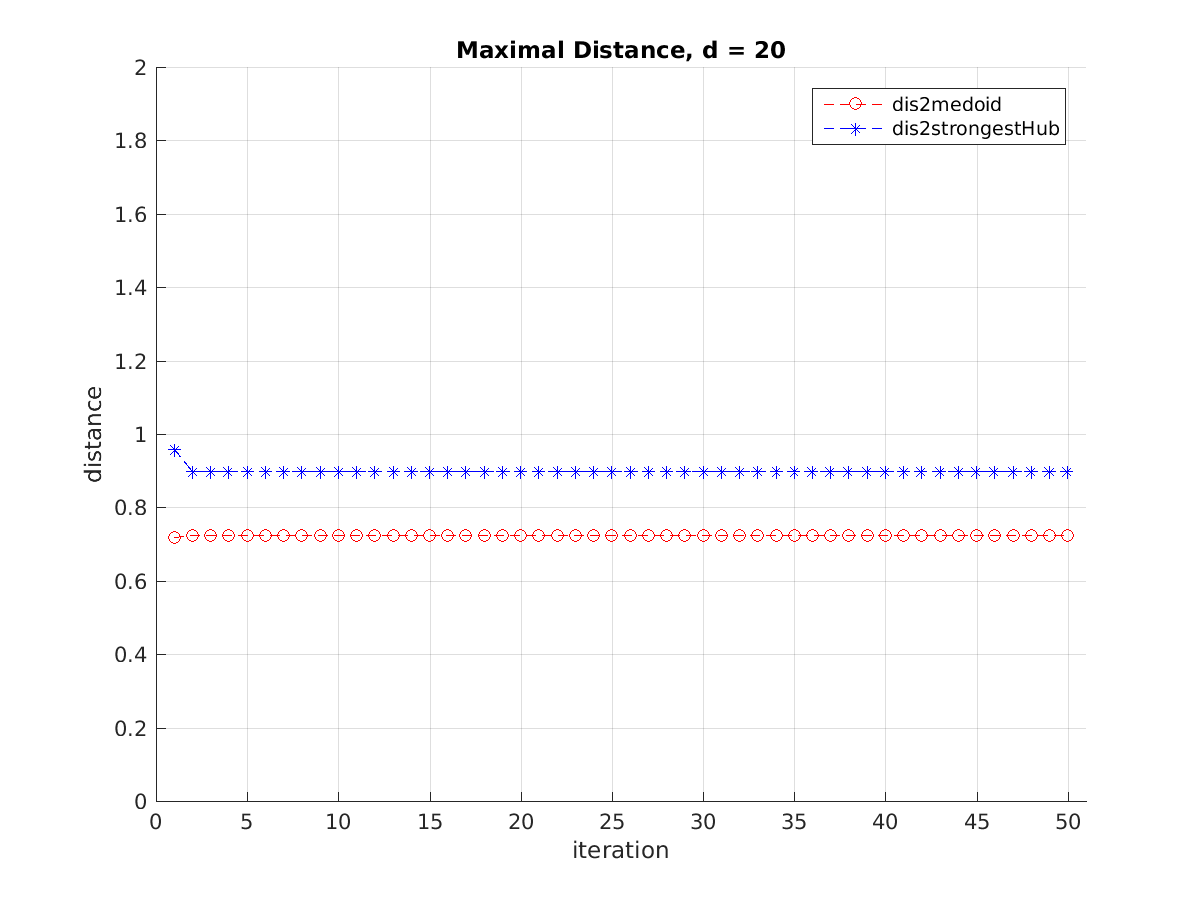
\includegraphics[width=0.4\textwidth]{FIGS/part1-synData/dim20_avg_max.png}
		}
		\hspace{5mm}
		\subfloat[Minimal dis, d = 30]{
			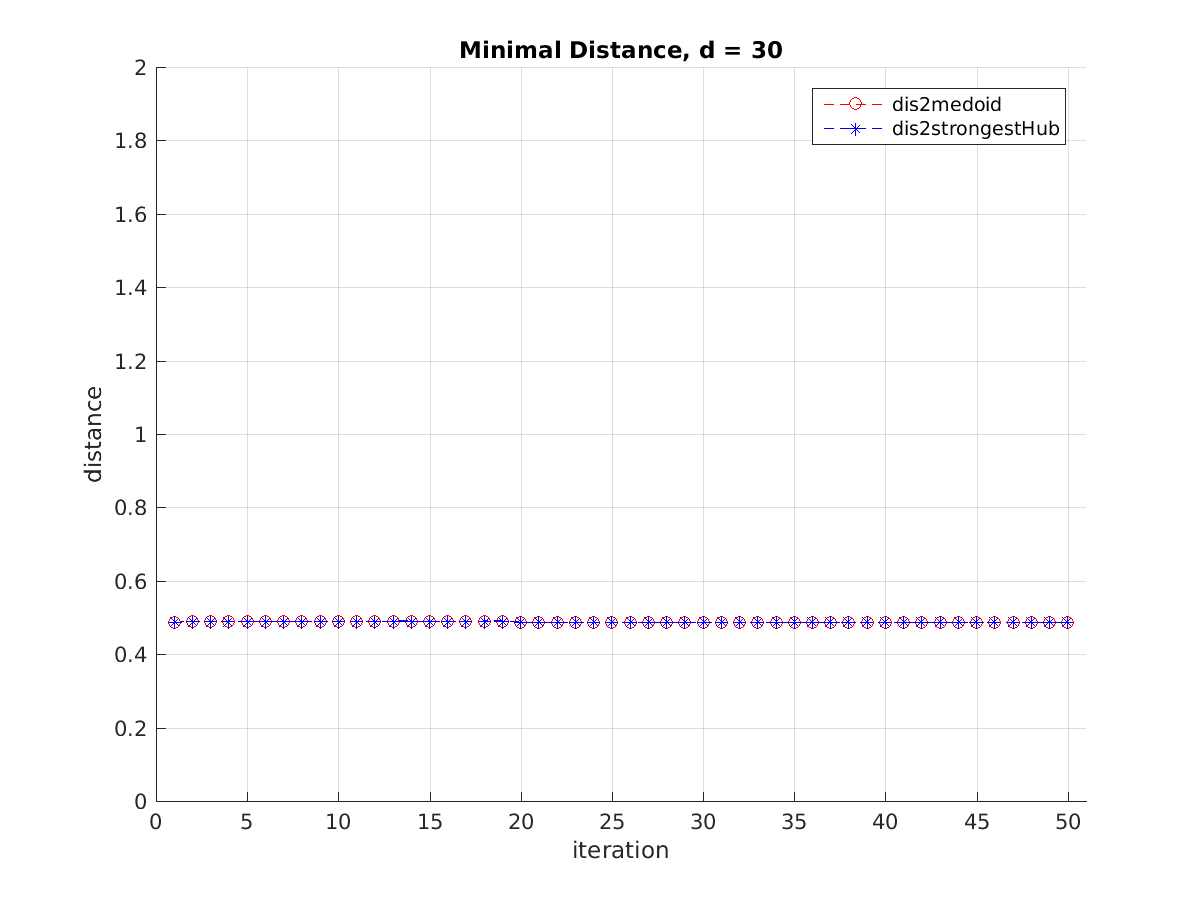
\includegraphics[width=0.4\textwidth]{FIGS/part1-synData/dim30_avg_min.png}
		}
		\hspace{5mm}
		\subfloat[Maximal dis, d = 30]{
			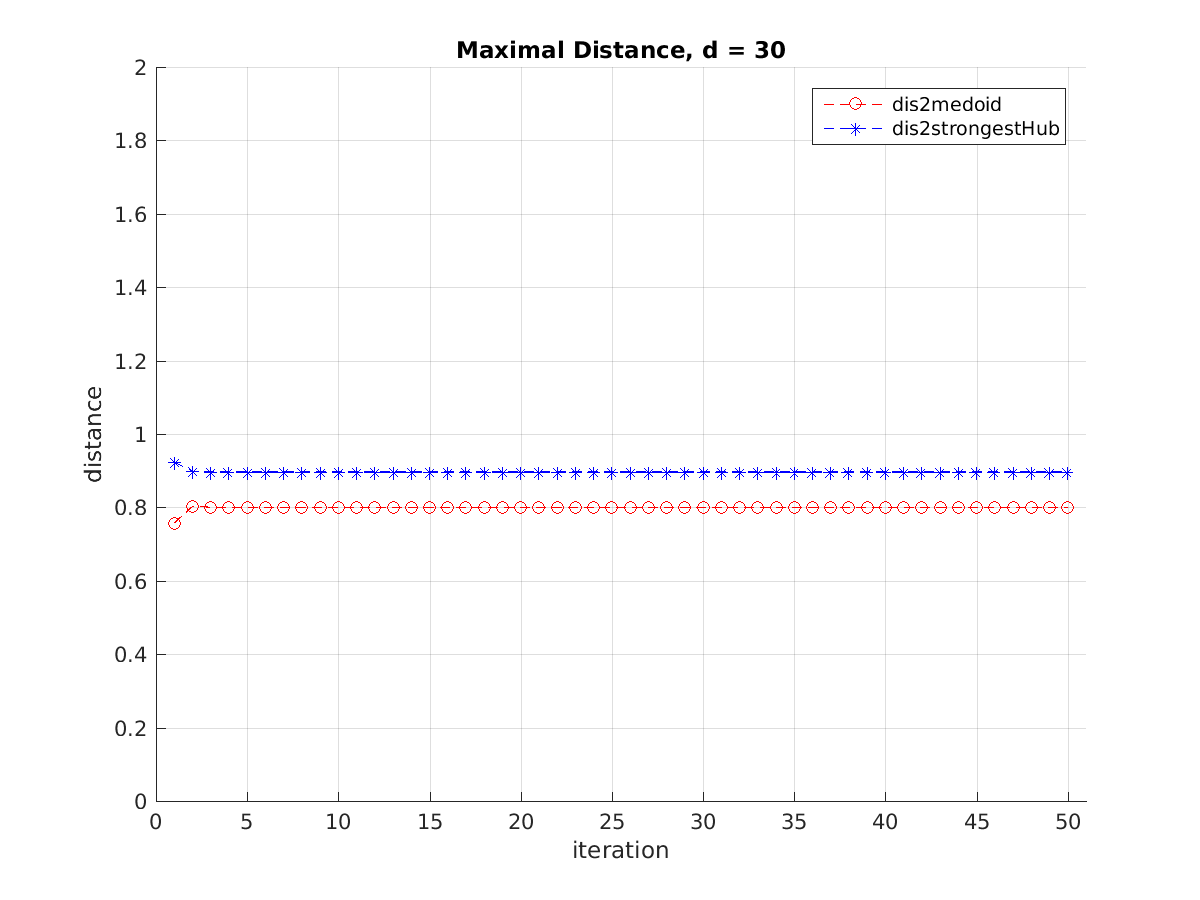
\includegraphics[width=0.4\textwidth]{FIGS/part1-synData/dim30_avg_max.png}
		}
		\hspace{5mm}
		\subfloat[Minimal dis, d = 50]{
			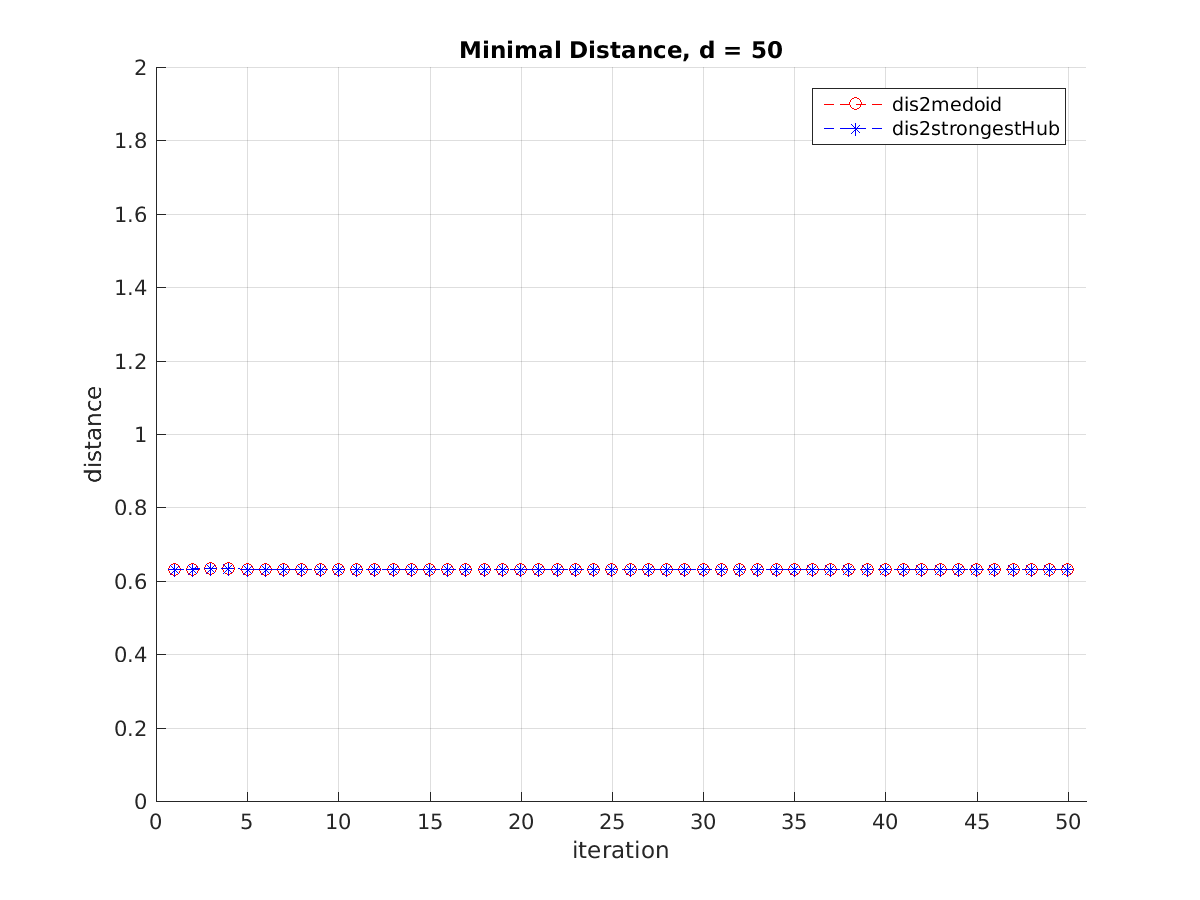
\includegraphics[width=0.4\textwidth]{FIGS/part1-synData/dim50_avg_min.png}
		}
		\hspace{5mm}
		\subfloat[Maximal dis, d = 50]{
			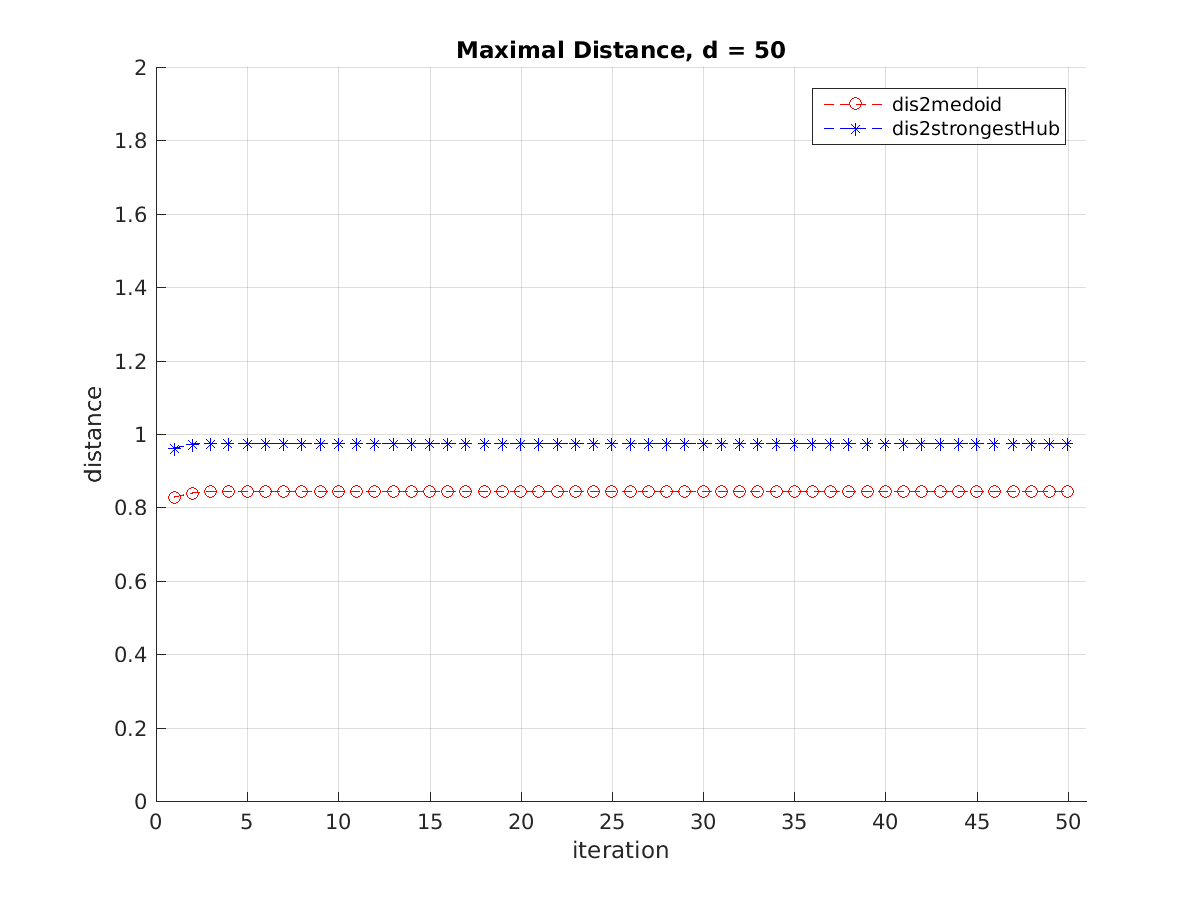
\includegraphics[width=0.4\textwidth]{FIGS/part1-synData/dim50_avg_max.png}
		}
		\hspace{5mm}
		\subfloat[Minimal dis, d = 100]{
			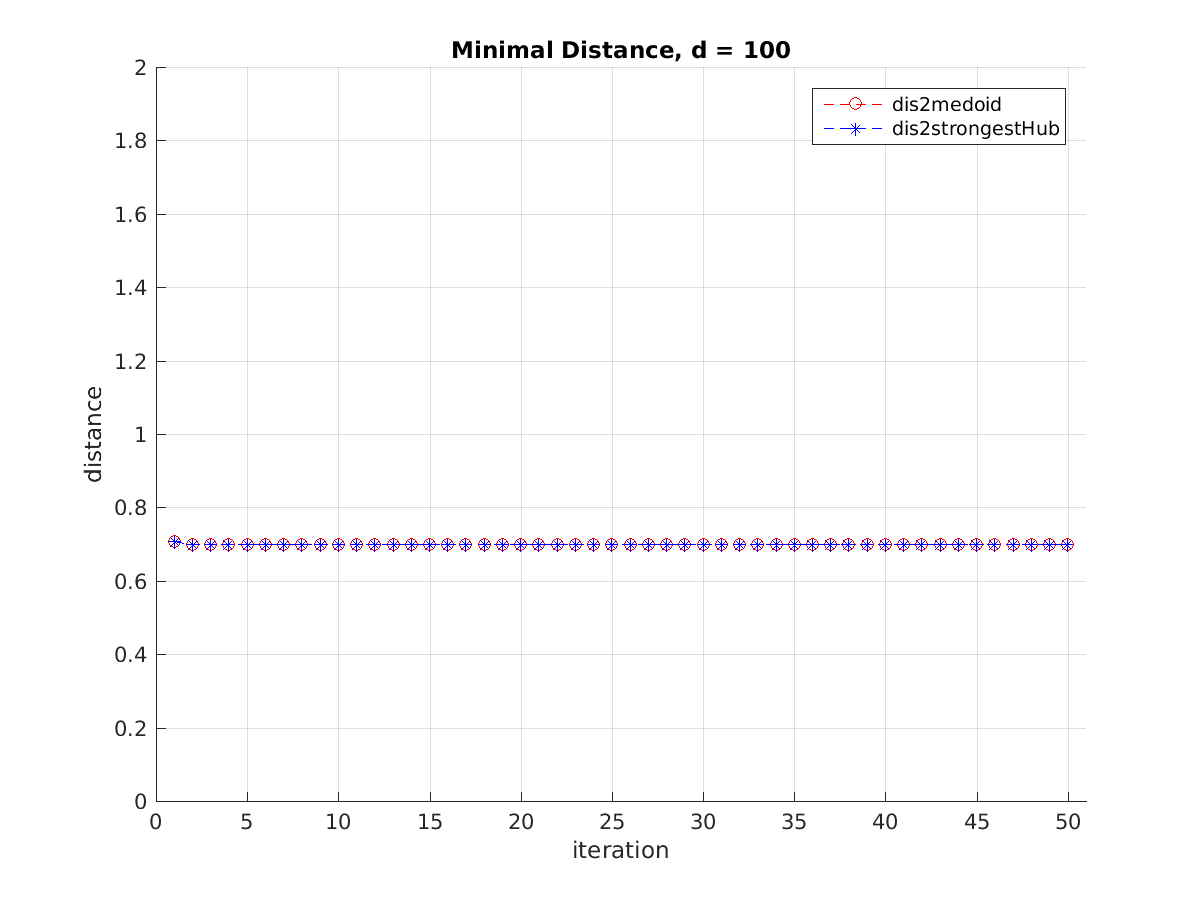
\includegraphics[width=0.4\textwidth]{FIGS/part1-synData/dim100_avg_min.png}
		}
		\hspace{5mm}
		\subfloat[Maximal dis, d = 100]{
			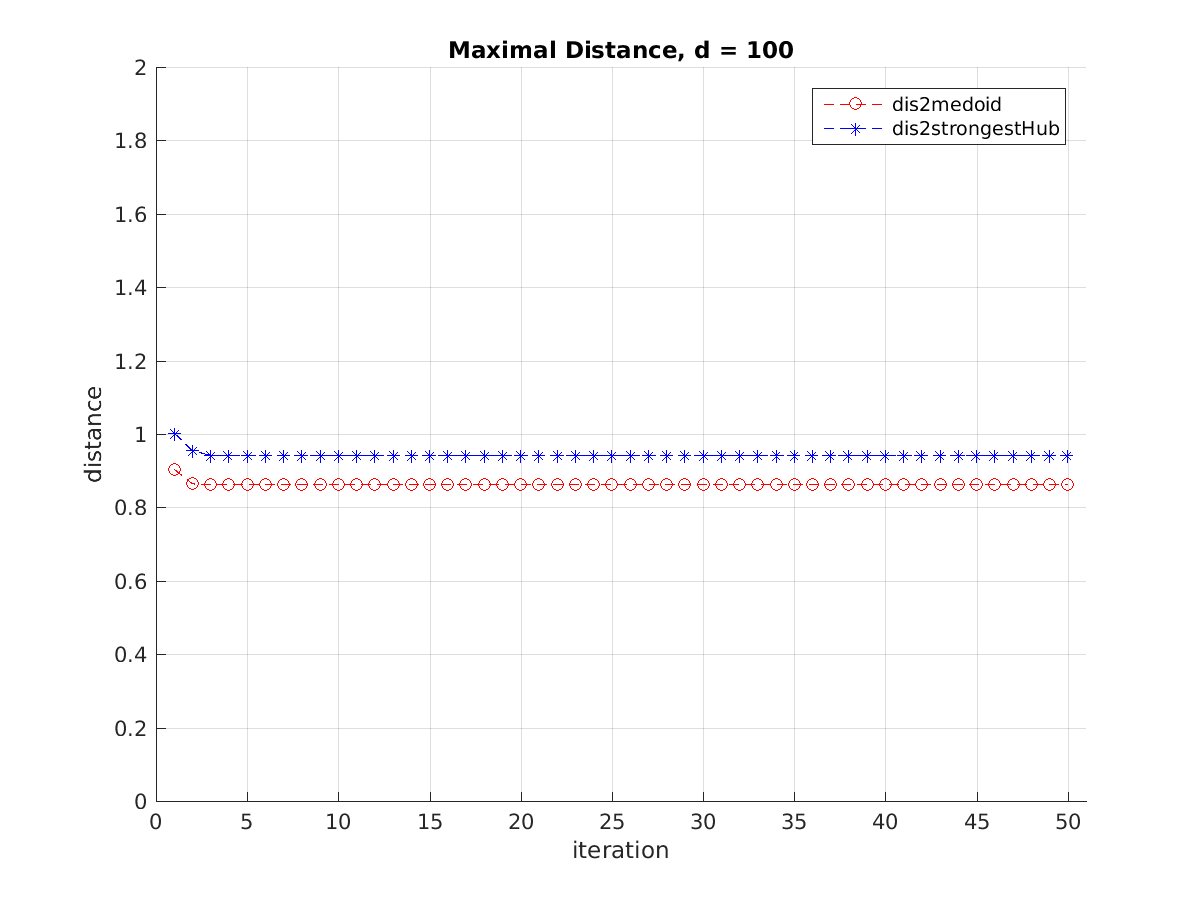
\includegraphics[width=0.4\textwidth]{FIGS/part1-synData/dim100_avg_max.png}
		}
	\caption{high-dim synthetic data results}
	\label{fig:syn2}
	\end{center}
\end{figure}
% real dataset min and max distances of lower dimension
\begin{figure}[ht]
	\begin{center}
		\subfloat[Minimal dis, Iris Dataset]{
			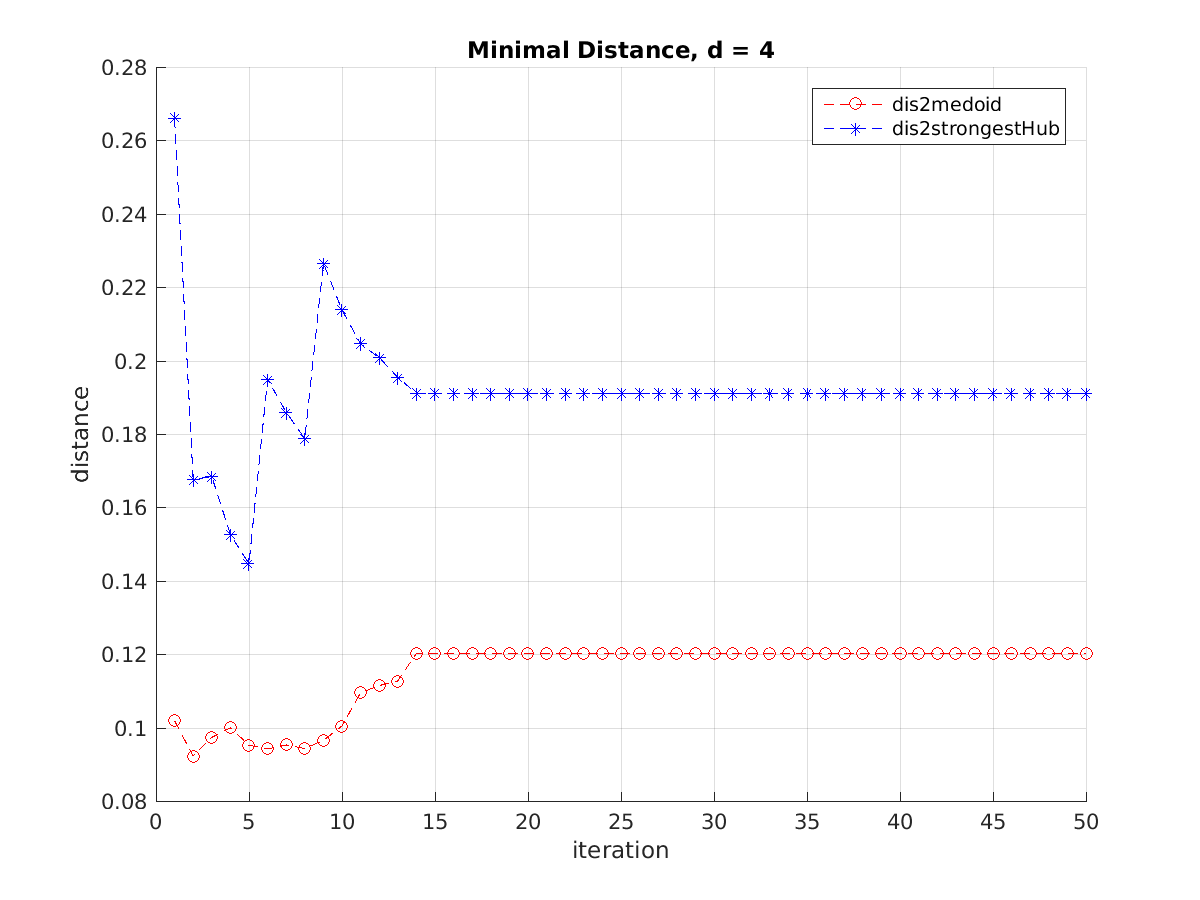
\includegraphics[width=0.4\textwidth]{FIGS/part1-realData/dim4_irisDataset_min.png}
		}
		\hspace{5mm}
		\subfloat[Maximal dis, Iris Dataset]{
			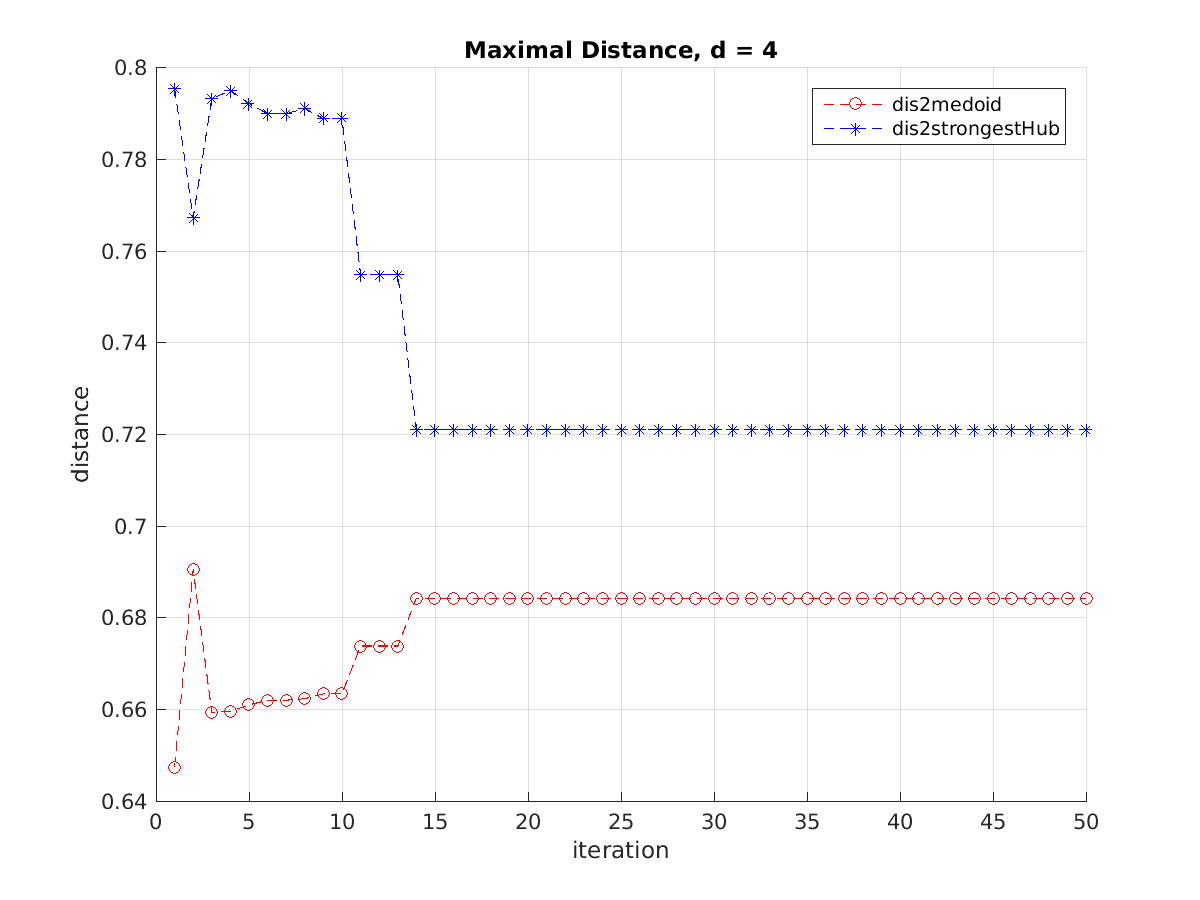
\includegraphics[width=0.4\textwidth]{FIGS/part1-realData/dim4_irisDataset_max.png}
		}
		\hspace{5mm}
		\subfloat[Minimal dis, Abalone Dataset]{
			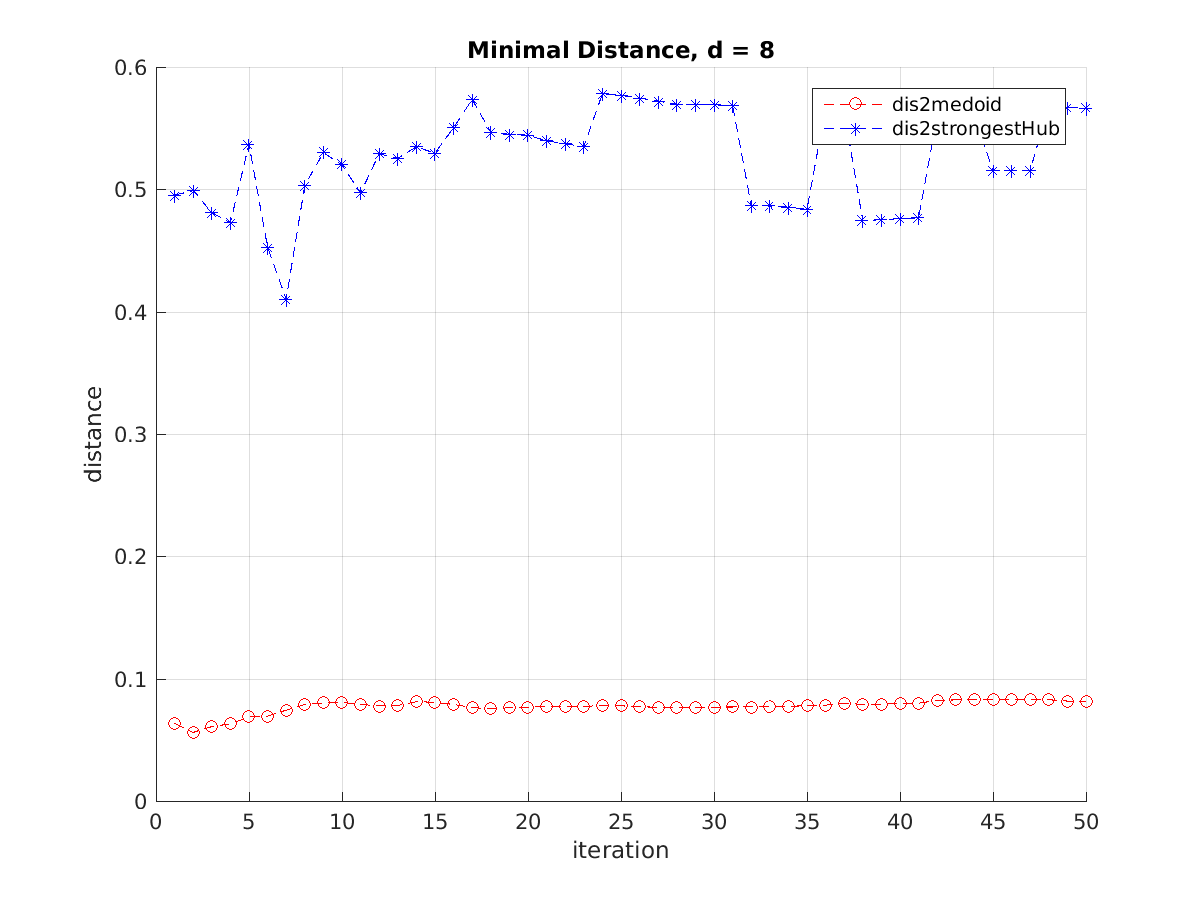
\includegraphics[width=0.4\textwidth]{FIGS/part1-realData/dim8_abaloneDataset_min.png}
		}
		\hspace{5mm}
		\subfloat[Maximal dis, Abalone Dataset]{
			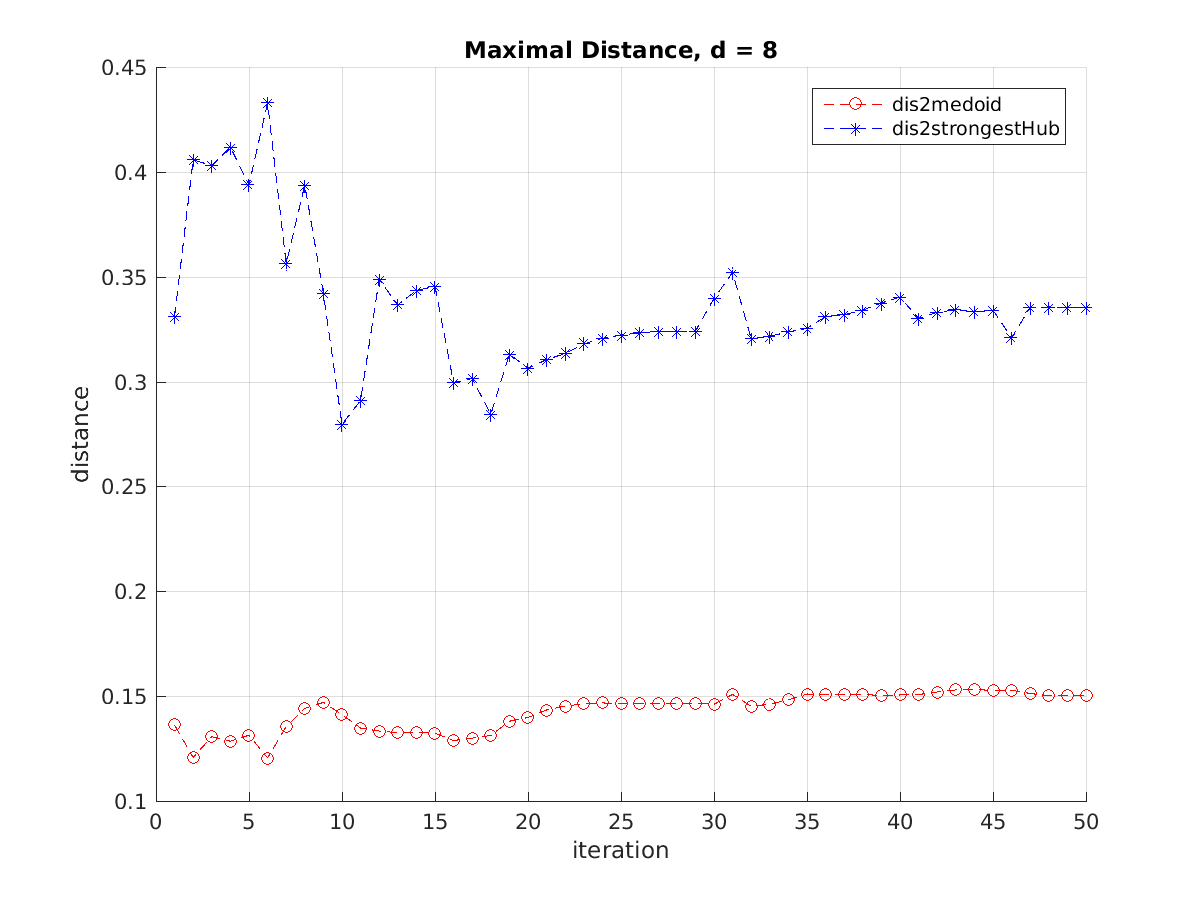
\includegraphics[width=0.4\textwidth]{FIGS/part1-realData/dim8_abaloneDataset_max.png}
		}
		\caption{low-dim real data results}
	\label{fig:real1}
	\end{center}
\end{figure}
% real dataset min and max distances of higher dimension
\begin{figure}[ht]
	\begin{center}
		\subfloat[Minimal dis, Wpbc Dataset]{
			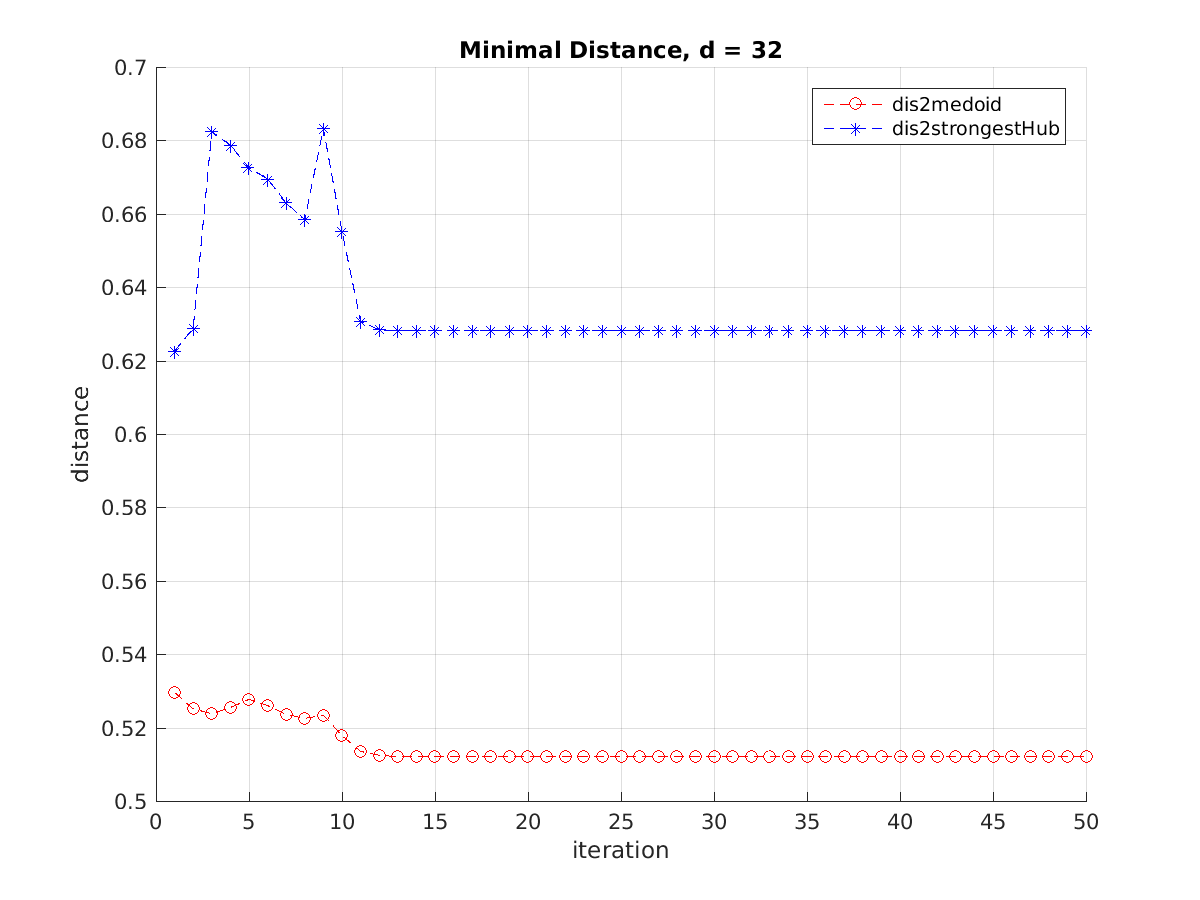
\includegraphics[width=0.4\textwidth]{FIGS/part1-realData/dim32_wpbcDataset_min.png}
		}
		\hspace{5mm}
		\subfloat[Maximal dis, Wpbc Dataset]{
			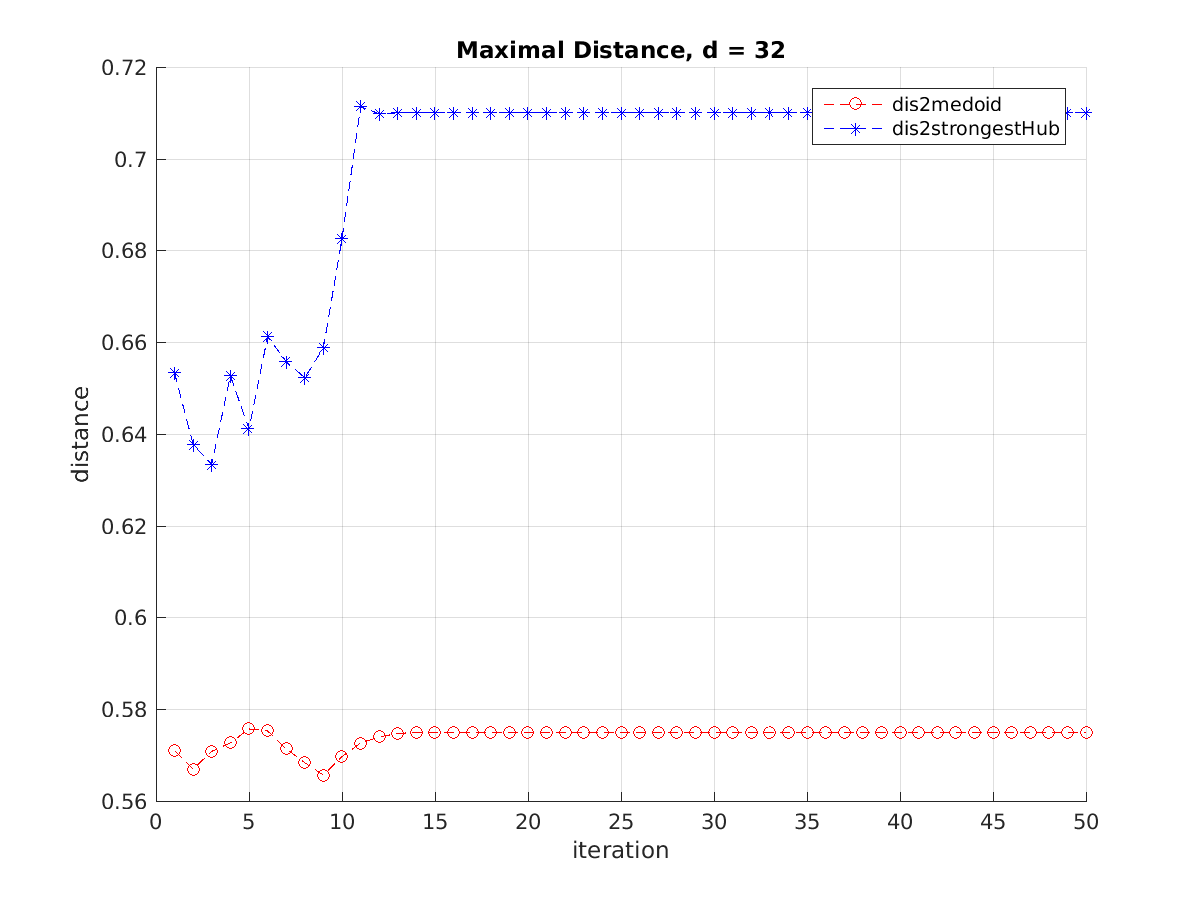
\includegraphics[width=0.4\textwidth]{FIGS/part1-realData/dim32_wpbcDataset_max.png}
		}
		\hspace{5mm}
		\subfloat[Minimal dis, Sonar Dataset]{
			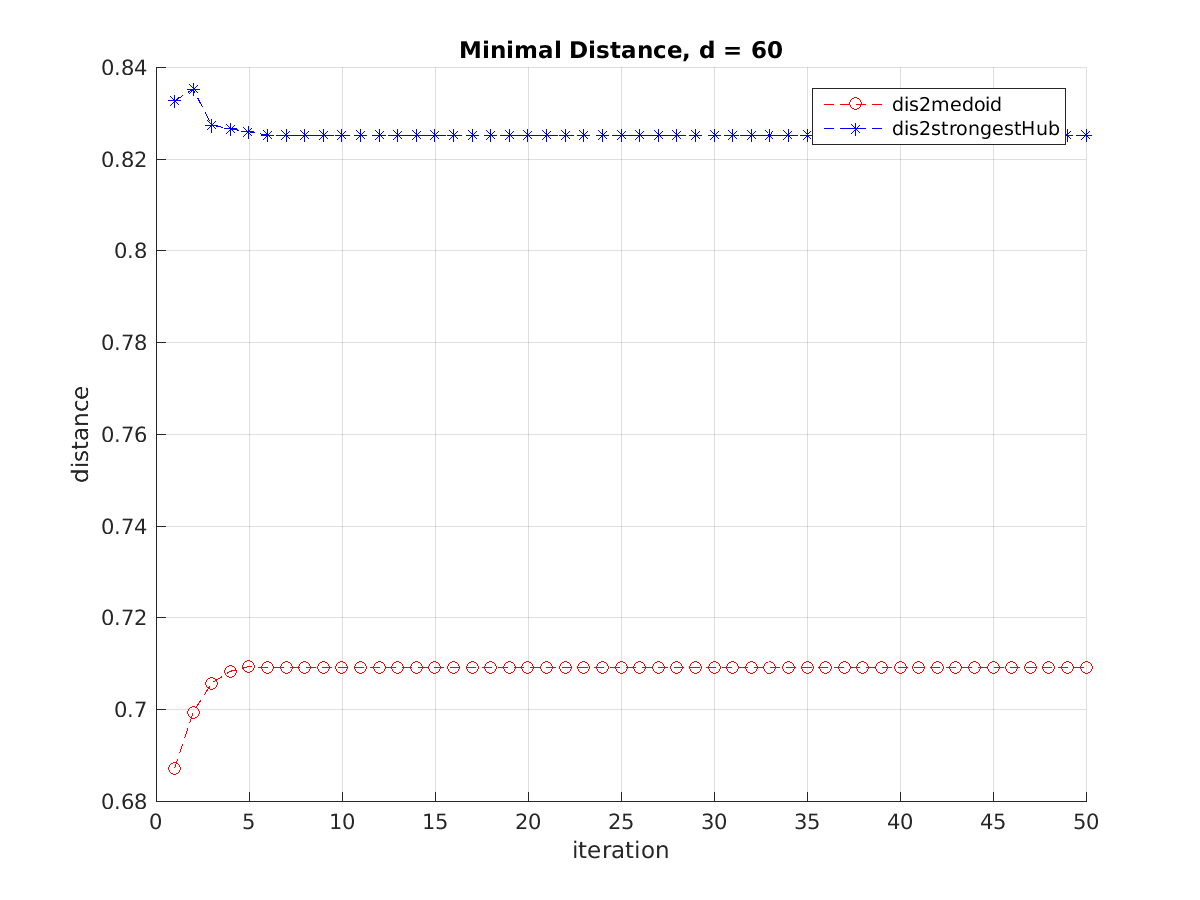
\includegraphics[width=0.4\textwidth]{FIGS/part1-realData/dim60_sonarDataset_min.png}
		}
		\hspace{5mm}
		\subfloat[Maximal dis, Sonar Dataset]{
			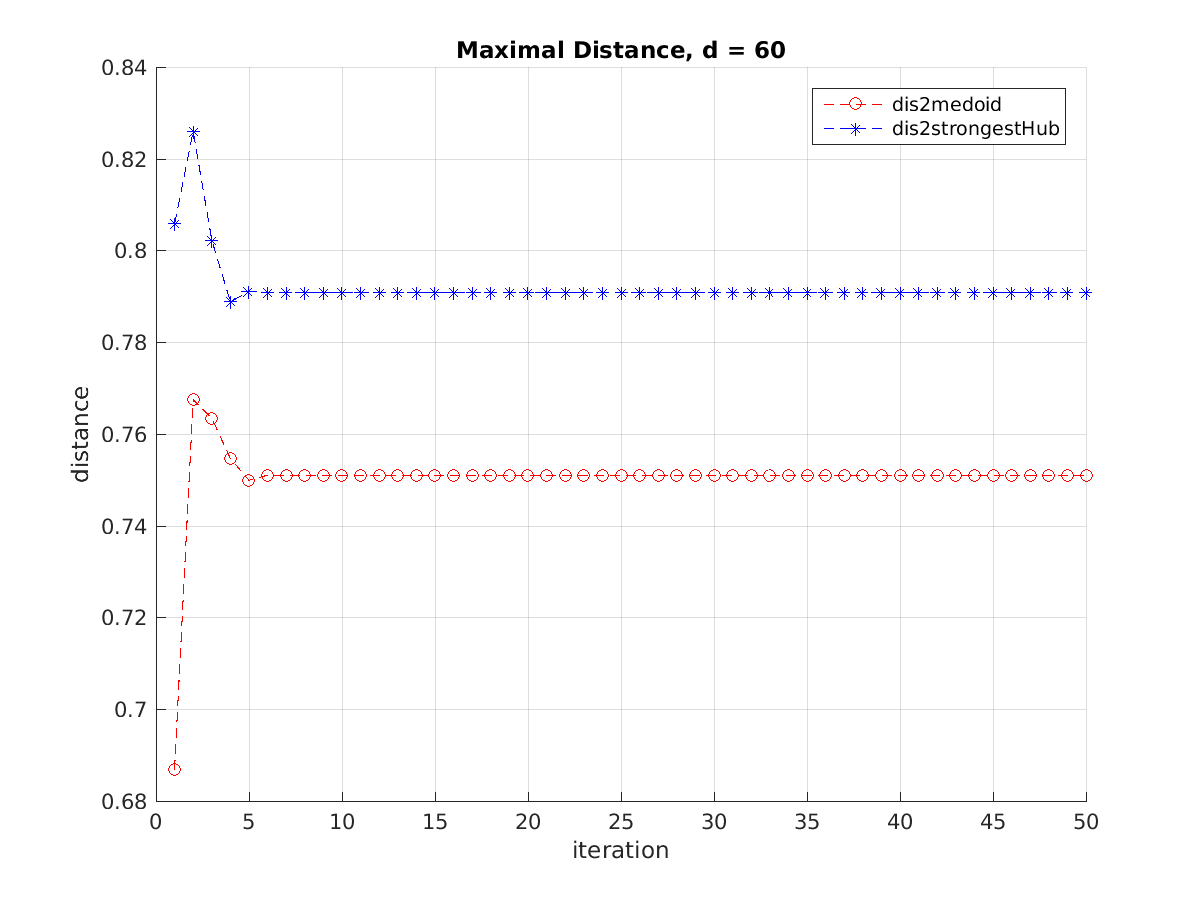
\includegraphics[width=0.4\textwidth]{FIGS/part1-realData/dim60_sonarDataset_max.png}
		}
		\hspace{5mm}
		\subfloat[Minimal dis, Hill Dataset]{
			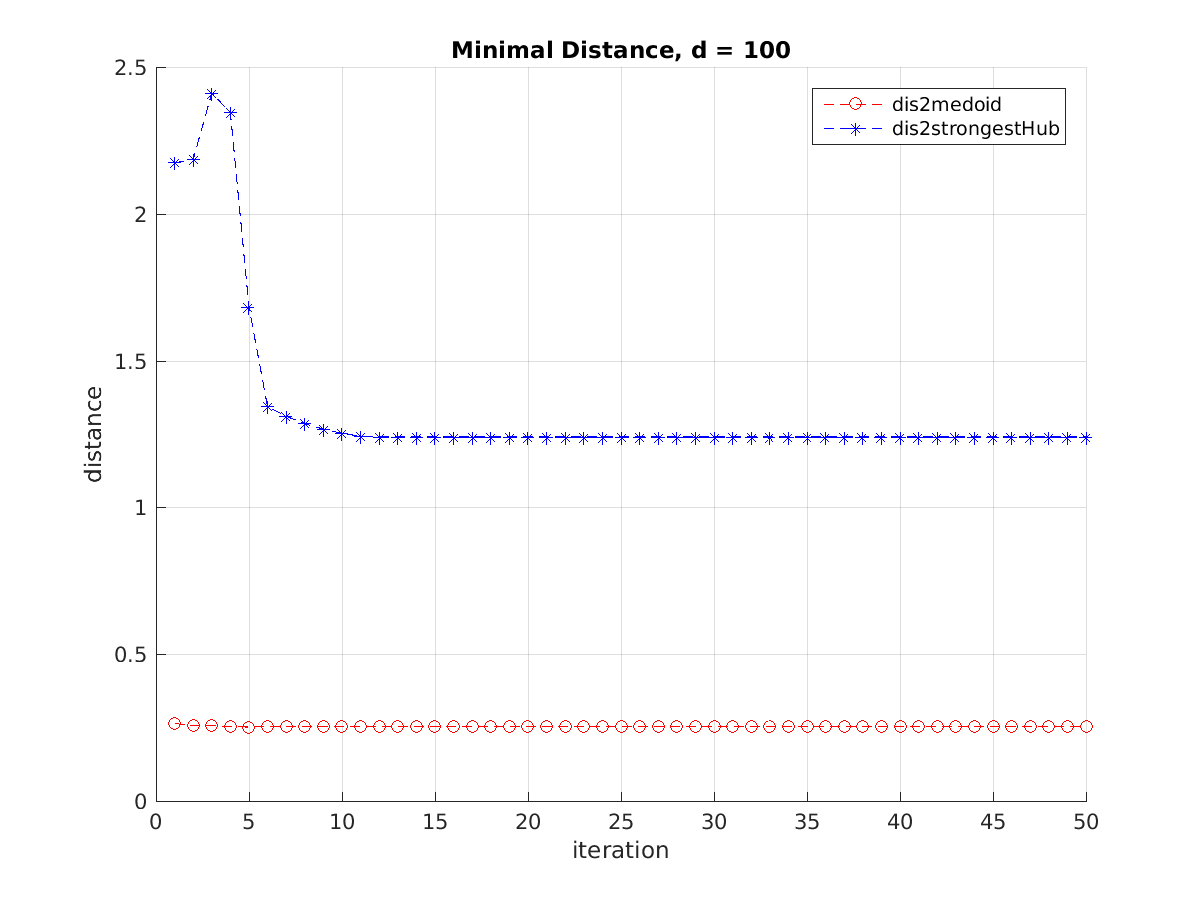
\includegraphics[width=0.4\textwidth]{FIGS/part1-realData/dim100_hillDataset_min.png}
		}
		\hspace{5mm}
		\subfloat[Maximal dis, Hill Dataset]{
			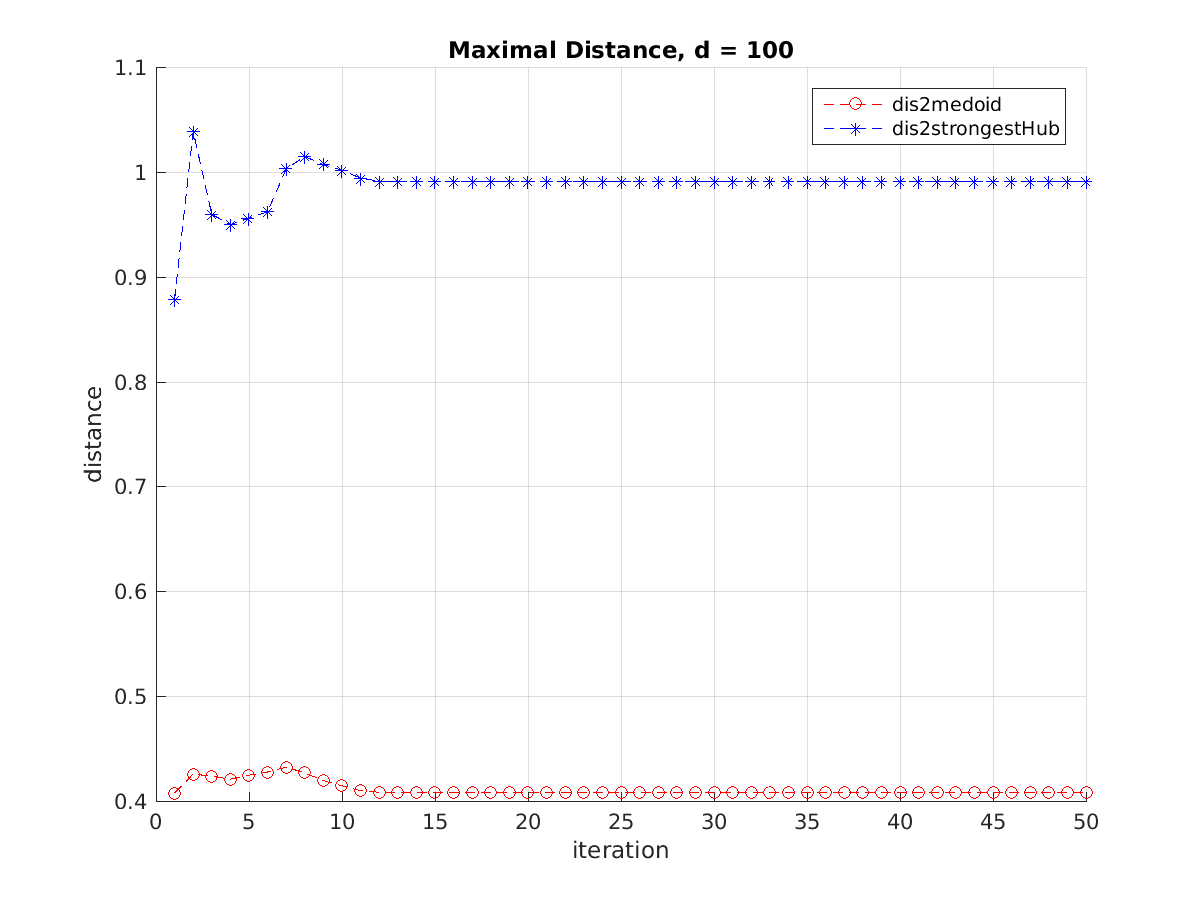
\includegraphics[width=0.4\textwidth]{FIGS/part1-realData/dim100_hillDataset_max.png}
		}
		\caption{high-dim real data results}
	\label{fig:real2}
	\end{center}
\end{figure}
%kdist graph
\begin{figure}[ht]
	\begin{center}
		\subfloat[Synthetic Dataset, d = 2]{
			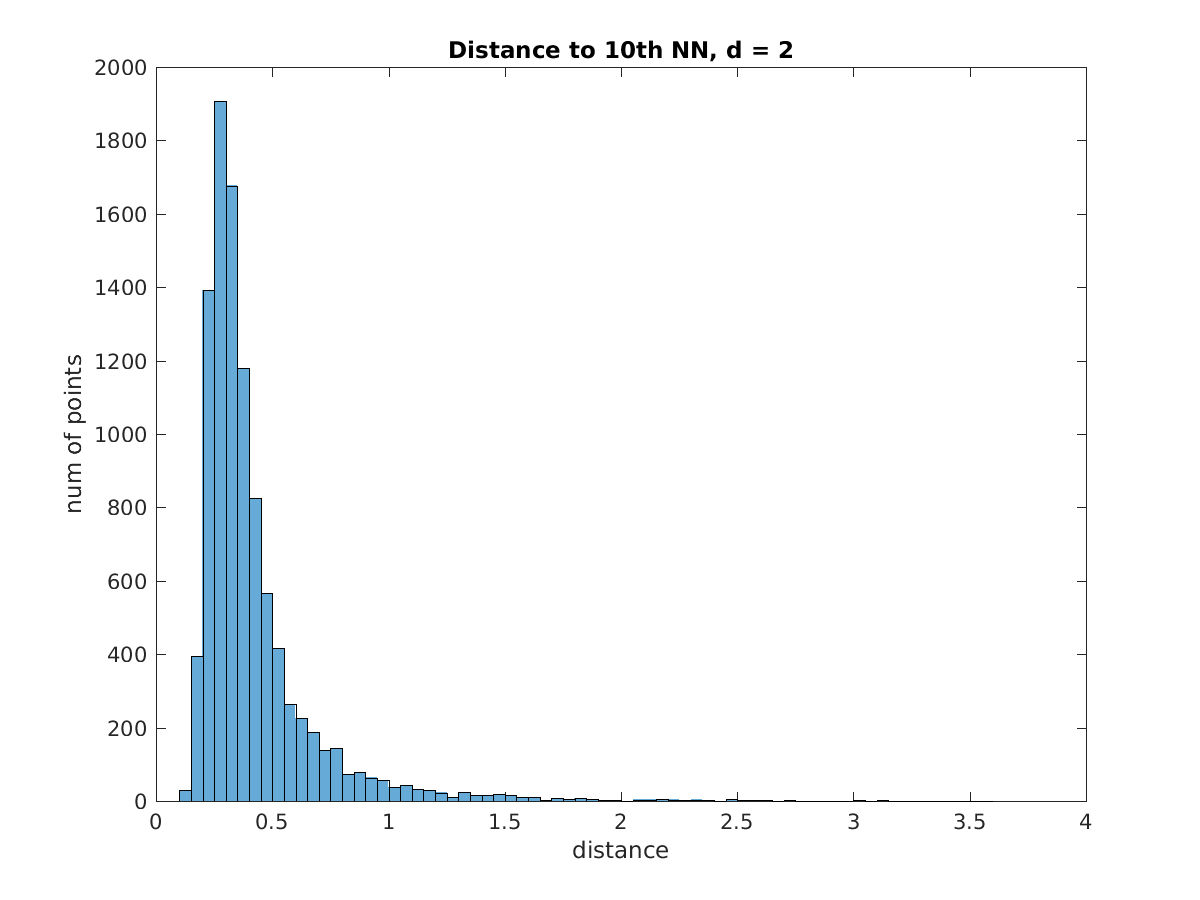
\includegraphics[width=0.4\textwidth]{FIGS/part2-synData/dim2_dis2NN_hist.png}
		}
		\hspace{5mm}
		\subfloat[Iris Dataset, d = 4]{
			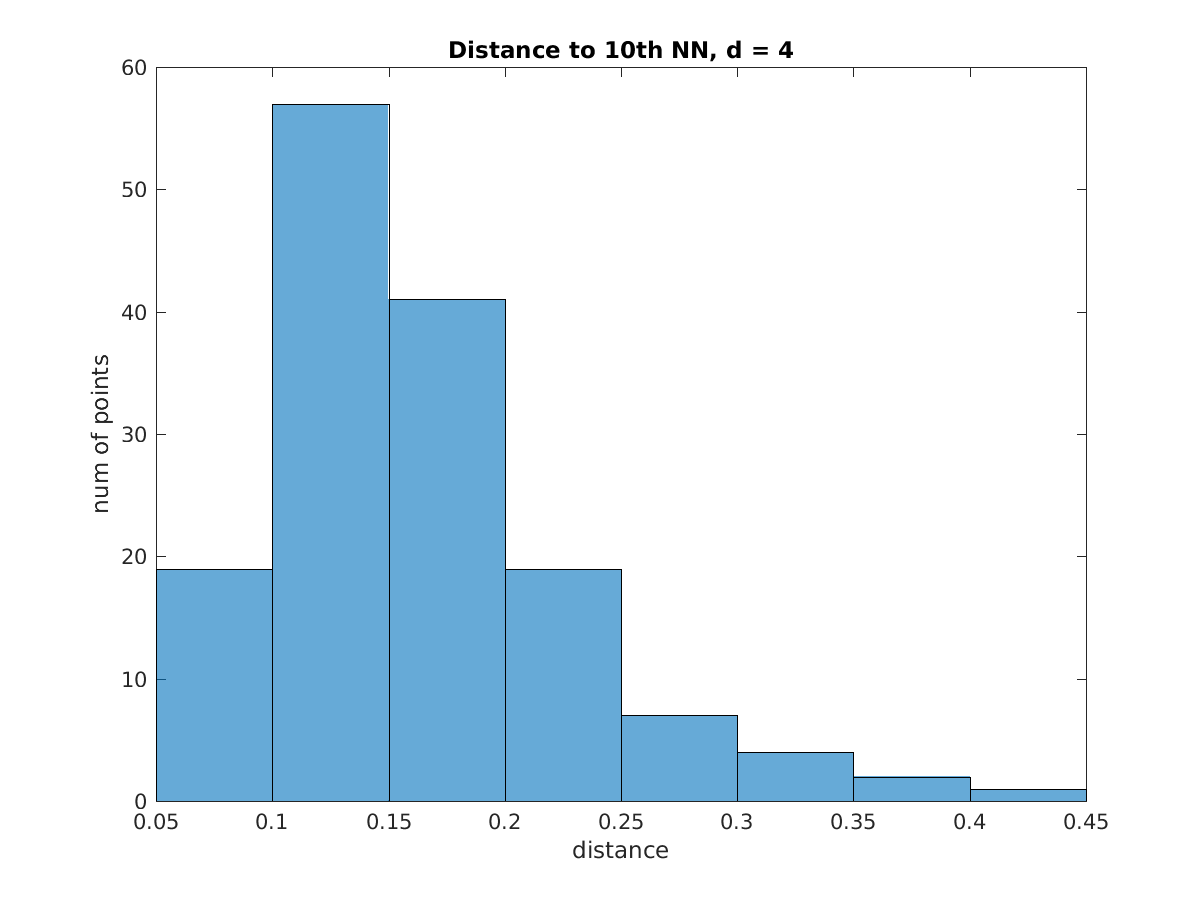
\includegraphics[width=0.4\textwidth]{FIGS/part2-realData/dim4_iris_dis2NN_hist.png}
		}
		\caption{kdist graph of low dimensional data}
		\label{fig:example_gm}
	\end{center}
\end{figure}
% table 2
\begin{table}
\begin{center}
	\begin{tabular}{||c c c c||}
	\hline
	Synthetic Datasets & $N_{a}$ of Noise Points& $N_{b}$ of Noise Points below Average & Percentage $\frac{N_{b}}{N_{a}}$\\[0.5ex]
	\hline
	\hline
	2-dim gm & 157 (from $10^4$ points) & 97 & $61.78\%$\\
	\hline
	5-dim gm & 121 (from $10^4$ points) & 95 & $78.51\%$\\
	\hline
	10-dim gm & 120 (from $10^4$ points) & 0 & $0\%$\\
	\hline
	20-dim gm & 121 (from $10^4$ points) & 0 & $0\%$\\
	\hline
	30-dim gm & 129 (from $10^4$ points) & 0 & $0\%$\\
	\hline
	50-dim gm & 110 (from $10^4$ points) & 0 & $0\%$\\
	\hline
	100-dim gm & 117 (from $10^4$ points) & 0 & $0\%$\\
	\hline
\end{tabular}
\caption{Compare DBSCAN noise points hubness score to the average on synthetic datasets}
\end{center}
\label{tab:noise1}
\end{table} 

\begin{table}
\begin{center}
	\begin{tabular}{||c c c c||}
	\hline
	Real Datasets & $N_{a}$ of Noise Points & $N_{b}$ of Noise Points below Average & Percentage $\frac{N_{b}}{N_{a}}$\\[0.5ex]
	\hline
	\hline
	Iris & 2 (from 150 points) & 0 & $0\%$\\
	\hline
	Abalone & 29 (from 4177 points) & 0 & $0\%$\\
	\hline
	Wpbg & 4 (from 198 points) & 0 & $0\%$\\
	\hline
	Sonar & 5 (from 208 points) & 0 & $0\%$\\
	\hline
	Hill & 4 (from 606 points) & 3 & $75\%$\\
	\hline
\end{tabular}
\caption{Compare DBSCAN noise points hubness score to the average on real datasets}
\end{center}
\label{tab:noise2}
\end{table} 


\section{Conclusion}

\section{Contribution}
Yimeng Li finished exploring the relation between hign-hubness points and cluster modoids. He also finished exploring the relation between low-hubness points and DBSCAN-detected noise points.

\bibliography{report}



\end{document}


